\thispagestyle{toancuabinone}
\pagestyle{toancuabi}
\everymath{\color{toancuabi}}
\blfootnote{$^*$\color{toancuabi}Nguồn: Câu lạc bộ Toán học Unicorn (UMC)}
\graphicspath{{../toancuabi/pic/}}
\begingroup
\AddToShipoutPicture*{\put(0,616){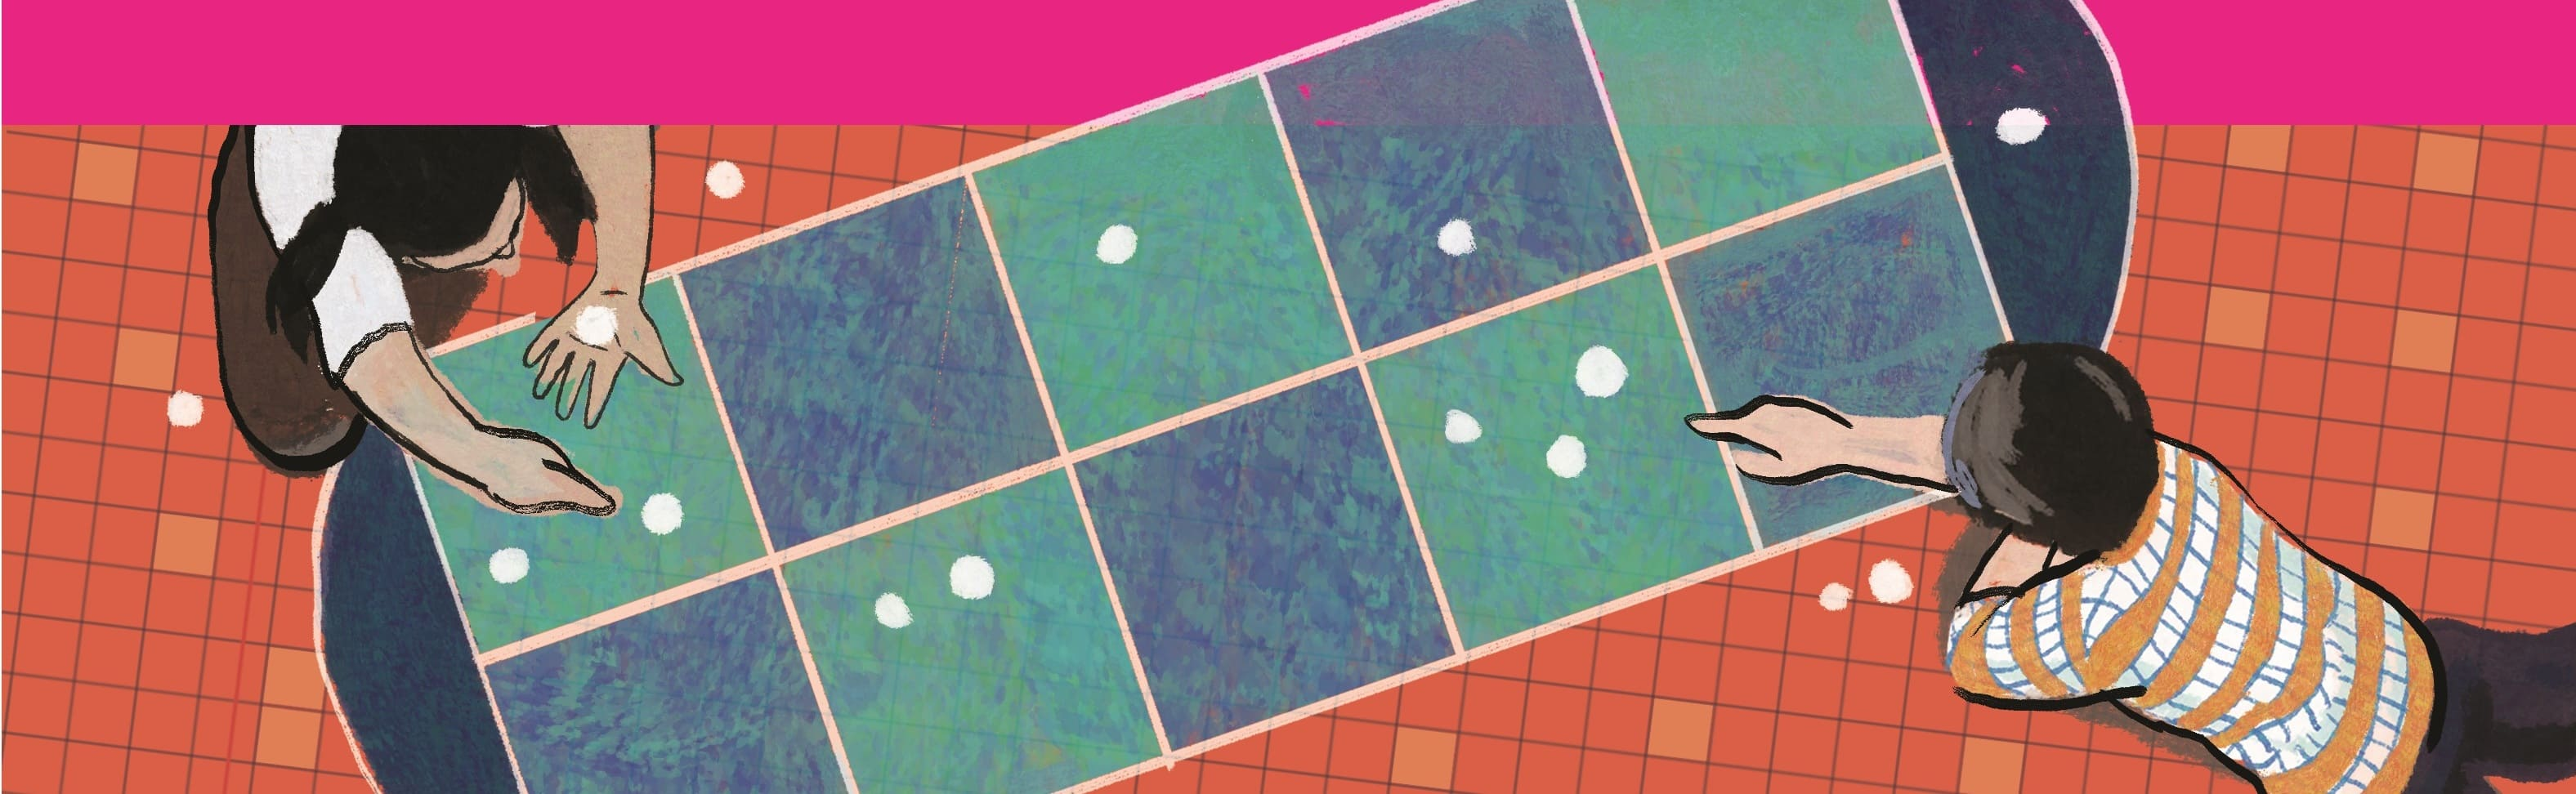
\includegraphics[width=19.3cm]{../bannertoancuabi}}}  
\AddToShipoutPicture*{\put(62,512){
\includegraphics[scale=1]{../tieude1.pdf}}}  
\centering
\endgroup
\vspace*{195pt} 

\definecolor{bulgarianrose}{rgb}{0.28, 0.02, 0.03}
\begin{multicols}{2}
	Trong số này, tạp chí Pi tiếp tục giới thiệu đến với bạn đọc đề thi tuyển sinh năm $2023-2024$ dành cho các bạn học sinh lớp $5$. Các bạn có thể thử sức làm của mình trong khoảng thời gian $90$ phút.
	\vskip 0.1cm
	\textbf{\color{toancuabi}Bài $\pmb1$.} 
	Dựa vào quy luật, hãy cho biết có bao nhiêu dấu thăng trong hình thứ tám của dãy hình sau.
	\begin{figure}[H]
		\vspace*{-5pt}
		\centering
		\captionsetup{labelformat= empty, justification=centering}
		\begin{tikzpicture}[cackithi,scale=0.3,node font=\scriptsize]
			\draw (0,0) grid (2,2);	
			\draw (3,0) grid (7,4);
			\draw (8,0) grid (14,6);
			\draw (15,0) grid (23,8);
			\draw (0.5,0.5) node {$\#$};
			\draw (1.5,0.5) node {$\#$};
			\draw (0.5,1.5) node {$\#$};
			\draw (3.5,0.5) node {$\#$};
			\draw (4.5,0.5) node {$\#$};
			\draw (5.5,0.5) node {$\#$};
			\draw (6.5,0.5) node {$\#$};
			\draw (3.5,1.5) node {$\#$};
			\draw (5.5,1.5) node {$\#$};
			\draw (4.5,2.5) node {$\#$};
			\draw (6.5,2.5) node {$\#$};
			\draw (3.5,3.5) node {$\#$};
			\draw (5.5,3.5) node {$\#$};
			\draw (8.5,0.5) node {$\#$};
			\draw (9.5,0.5) node {$\#$};
			\draw (10.5,0.5) node {$\#$};
			\draw (11.5,0.5) node {$\#$};
			\draw (12.5,0.5) node {$\#$};
			\draw (13.5,0.5) node {$\#$};
			\draw (8.5,1.5) node {$\#$};
			\draw (10.5,1.5) node {$\#$};
			\draw (12.5,1.5) node {$\#$};
			\draw (9.5,2.5) node {$\#$};
			\draw (11.5,2.5) node {$\#$};
			\draw (13.5,2.5) node {$\#$};
			\draw (8.5,3.5) node {$\#$};
			\draw (10.5,3.5) node {$\#$};
			\draw (12.5,3.5) node {$\#$};
			\draw (9.5,4.5) node {$\#$};
			\draw (11.5,4.5) node {$\#$};
			\draw (13.5,4.5) node {$\#$};
			\draw (8.5,5.5) node {$\#$};
			\draw (10.5,5.5) node {$\#$};
			\draw (12.5,5.5) node {$\#$};
			\draw (15.5,0.5) node {$\#$};
			\draw (16.5,0.5) node {$\#$};
			\draw (17.5,0.5) node {$\#$};
			\draw (18.5,0.5) node {$\#$};
			\draw (19.5,0.5) node {$\#$};
			\draw (20.5,0.5) node {$\#$};
			\draw (21.5,0.5) node {$\#$};
			\draw (22.5,0.5) node {$\#$};
			\draw (15.5,0.5) node {$\#$};
			\draw (17.5,0.5) node {$\#$};
			\draw (19.5,0.5) node {$\#$};
			\draw (21.5,0.5) node {$\#$};
			\draw (16.5,1.5) node {$\#$};
			\draw (18.5,1.5) node {$\#$};
			\draw (20.5,1.5) node {$\#$};
			\draw (22.5,1.5) node {$\#$};
			\draw (15.5,2.5) node {$\#$};
			\draw (17.5,2.5) node {$\#$};
			\draw (19.5,2.5) node {$\#$};
			\draw (21.5,2.5) node {$\#$};
			\draw (16.5,3.5) node {$\#$};
			\draw (18.5,3.5) node {$\#$};
			\draw (20.5,3.5) node {$\#$};
			\draw (22.5,3.5) node {$\#$};
			\draw (15.5,4.5) node {$\#$};
			\draw (17.5,4.5) node {$\#$};
			\draw (19.5,4.5) node {$\#$};
			\draw (21.5,4.5) node {$\#$};
			\draw (16.5,5.5) node {$\#$};
			\draw (18.5,5.5) node {$\#$};
			\draw (20.5,5.5) node {$\#$};
			\draw (22.5,5.5) node {$\#$};
			\draw (15.5,6.5) node {$\#$};
			\draw (17.5,6.5) node {$\#$};
			\draw (19.5,6.5) node {$\#$};
			\draw (21.5,6.5) node {$\#$};
			\draw (16.5,7.5) node {$\#$};
			\draw (18.5,7.5) node {$\#$};
			\draw (20.5,7.5) node {$\#$};
			\draw (22.5,7.5) node {$\#$};
			\draw (1,-1) node {Hình $1$};
			\draw (5,-1) node {Hình $2$};
			\draw (11,-1) node {Hình $3$};
			\draw (19,-1) node {Hình $4$};
		\end{tikzpicture}
		\vspace*{-15pt}
	\end{figure}
	\textbf{\color{toancuabi}Bài $\pmb2$.} Bạn Tâm xếp các số $0, 0, 1, 1, 2, 2, 2, 3$ vào các ô vuông trong hình dưới đây (mỗi ô một số) để tạo thành phép trừ của hai số có $4$ chữ số. Hỏi hiệu nhận được lớn nhất có thể là bao nhiêu? 
	\vskip 0.1cm
	Chú ý: \textit{một số có bốn chữ số không được bắt đầu bằng số $0$.}
	\begin{figure}[H]
		\vspace*{-5pt}
		\centering
		\captionsetup{labelformat= empty, justification=centering}
		\begin{tikzpicture}[toancuabi,scale=0.77]
			\draw (0,0) grid (4,1);
			\draw (4.5,0.5) node {$-$};
			\draw (5,0) grid (9,1);
		\end{tikzpicture}
		\vspace*{-10pt}
	\end{figure}
	\textbf{\color{toancuabi}Bài $\pmb3$.} Diện tích của hình được tô đậm bên dưới bằng bao nhiêu?
	\begin{figure}[H]
		\vspace*{5pt}
		\centering
		\captionsetup{labelformat= empty, justification=centering}
		\definecolor{zzttqq}{rgb}{0.6,0.2,0.}
		\begin{tikzpicture}[toancuabi, scale=0.9]
			\fill[color=cackithi,fill=cackithi!40] (1.,0.) -- (2.,5.) -- (3.,0.) -- cycle;
			\fill[color=zzttqq,fill=cackithi!40] (1.,0.) -- (4.,5.) -- (3.,0.) -- (0.,5.) -- cycle;
			\draw  (1.,0.)-- (2.,5.);
			\draw  (2.,5.)-- (3.,0.);
			\draw  (3.,0.)-- (1.,0.);
			\draw  (1.,0.)-- (4.,5.);
			\draw  (4.,5.)-- (3.,0.);
			\draw  (3.,0.)-- (0.,5.);
			\draw  (0.,5.)-- (1.,0.);
			\draw[dashed]  (-1.,5.)-- (5.,5.);
			\draw[dashed]  (-1.,2.5)-- (5.,2.5);
			\draw[dashed]  (-1.,0.)-- (5.,0.);
			\draw[-stealth]  (4.5,5.)-- (4.5,2.5);
			\draw[-stealth]  (4.5,2.5)-- (4.5,0.);
			\draw[-stealth]  (1,-0.4)-- (3.,-0.4);
			
			\draw[-stealth]  (4.5,2.5) -- (4.5,5.);
			\draw[-stealth]  (4.5,0.) -- (4.5,2.5);
			\draw[-stealth]  (3.,-0.4) -- (1,-0.4);
			\draw[color=black] (4.21498164902576,3.87946061896495) node {$5$};
			\draw[color=black] (4.143071467449243,1.3626042637868525) node {$5$};
			\draw[color=black] (2.039698656336115,-0.709930933849792) node {$4$};
		\end{tikzpicture}
		\vspace*{-10pt}
	\end{figure}
	\textbf{\color{toancuabi}Bài $\pmb4$.} Trong bảng ô vuông cỡ $4\times 4$ có điền các số khác $0$ sao cho tích của $4$ số trong mỗi hàng, mỗi cột đều bằng nhau. Cho biết các số trong $9$ ô như hình vẽ, hỏi số ở ô có dấu $*$ bằng bao nhiêu?
	\begin{figure}[H]
		\vspace*{-5pt}
		\centering
		\captionsetup{labelformat= empty, justification=centering}
		\begin{tikzpicture}[toancuabi, node font=\small]
			\draw (0,0) grid (4,4);
			\draw (0.5,0.5) node {$32$};
			\draw (0.5,1.5) node {$4$};
			\draw (0.5,3.5) node {$\dfrac{1}{2}$};
			\draw (1.5,1.5) node {$1$};
			\draw (1.5,2.5) node {$4$};
			\draw (1.5,3.5) node {$32$};
			\draw (2.5,0.5) node {$*$};
			\draw (3.5,0.5) node {$16$};
			\draw (2.5,2.5) node {$8$};
			\draw (3.5,2.5) node {$2$};
		\end{tikzpicture}
		\vspace*{-5pt}
	\end{figure}
	\textbf{\color{toancuabi}Bài $\pmb5$.} Khu vườn của gia đình Tâm được minh họa bằng hình chữ nhật trong hình dưới đây. Biết rằng khu vườn có diện tích $120 \,m^2$ và được chia thành ba luống hình chữ nhật. Phần trồng hoa rộng $2\,m$, diện tích $20 \,m^2$, phần trồng dâu rộng $3\, m$. Hỏi diện tích phần trồng rau là bao nhiêu?
	\begin{figure}[H]
		\vspace*{-5pt}
		\centering
		\captionsetup{labelformat= empty, justification=centering}
		\begin{tikzpicture}[scale=0.4,toancuabi]
			\draw (0,0) rectangle (12,10);
			\draw (2,0) -- (2,10) (2,3) -- (12,3);
			\draw (1,10) node[below] {$2\,m$};
			\draw (1,5) node {Hoa};
			\draw (7,1.5) node {Dâu};
			\draw (7,6.5) node {Rau};
			\draw (12,1.5) node[right] {$3\,m$};
		\end{tikzpicture}
		\vspace*{-5pt}
	\end{figure}
	\textbf{\color{toancuabi}Bài $\pmb6$.} Ba bạn An, Bình, Chi chia đều nhau $30$ chiếc kẹo. An ăn một số chiếc kẹo; Bình ăn một số kẹo bằng với số kẹo mà An còn; Chi ăn số kẹo bằng với tổng số kẹo mà An và Bình đã ăn. Hỏi còn lại bao nhiêu chiếc kẹo?
	\vskip 0.1cm
	\textbf{\color{toancuabi}Bài $\pmb7$.} Một bác nông dân chở một xe ô tô quất cảnh ra chợ Tết để bán. Sau khi bán hết cây quất cuối cùng với giá $230$ nghìn đồng, bác tính nhẩm lại thấy mình đã bán số cây quất với giá trung bình là $245$ nghìn đồng/cây. Nhưng người mua cây quất cuối quay trở lại và chỉ cho bác thấy cành quất bị rụng quá nhiều lá, nên ông ta chỉ đồng ý mua với giá $158$ nghìn đồng. Bác chấp thuận và bán cây quất đó. Khi nhẩm tính lại, bác nông dân thấy giá trung bình của xe quất bây giờ là $242$ nghìn đồng. Hỏi bác đã bán được bao nhiêu cây quất?
	\vskip 0.1cm
	\columnbreak
	\textbf{\color{toancuabi}Bài $\pmb8$.} Có bao nhiêu cách xếp $5$ viên bi giống hệt nhau vào các ô hình vuông ở hình vẽ sau sao cho mỗi ô có không quá $1$ viên bi và không có $2$ viên bi nào trên cùng $1$ hàng hoặc $1$ cột?
	\begin{figure}[H]
		\vspace*{-10pt}
		\centering
		\captionsetup{labelformat= empty, justification=centering}
		\begin{tikzpicture}[toancuabi,scale=0.8]
			\draw  (0.,1.)-- (5.,1.);
			\draw  (5.,1.)-- (5.,4.);
			\draw  (5.,4.)-- (1.,4.);
			\draw  (1.,4.)-- (1.,3.);
			\draw  (1.,3.)-- (0.,3.);
			\draw  (0.,3.)-- (0.,1.);
			\draw  (1.,1.)-- (1.,3.);
			\draw  (1.,2.)-- (5.,2.);
			\draw  (5.,3.)-- (1.,3.);
			\draw  (1.,4.)-- (1.,5.);
			\draw  (1.,5.)-- (2.,5.);
			\draw  (2.,5.)-- (2.,1.);
			\draw  (3.,1.)-- (3.,6.);
			\draw  (3.,6.)-- (4.,6.);
			\draw  (4.,6.)-- (4.,1.);
			\draw  (0.,2.)-- (1.,2.);
			\draw  (3.,5.)-- (4.,5.);
			
			\draw [fill=cackithi!40] (0.,1.) circle (2.0pt);
			\draw [fill=cackithi!40] (5.,1.) circle (2.0pt);
			\draw [fill=cackithi!40] (5.,4.) circle (2.0pt);
			\draw [fill=cackithi!40] (1.,4.) circle (2.0pt);
			\draw [fill=cackithi!40] (1.,3.) circle (2.0pt);
			\draw [fill=cackithi!40] (0.,3.) circle (2.0pt);
			\draw [fill=cackithi!40] (1.,1.) circle (2.0pt);
			\draw [fill=cackithi!40] (1.,2.) circle (2.0pt);
			\draw [fill=cackithi!40] (5.,2.) circle (2.0pt);
			\draw [fill=cackithi!40] (5.,3.) circle (2.0pt);
			\draw [fill=cackithi!40] (1.,5.) circle (2.0pt);
			\draw [fill=cackithi!40] (2.,5.) circle (2.0pt);
			\draw [fill=cackithi!40] (2.,1.) circle (2.0pt);
			\draw [fill=cackithi!40] (3.,1.) circle (2.0pt);
			\draw [fill=cackithi!40] (3.,6.) circle (2.0pt);
			\draw [fill=cackithi!40] (4.,6.) circle (2.0pt);
			\draw [fill=cackithi!40] (4.,1.) circle (2.0pt);
			\draw [fill=cackithi!40] (2.,4.) circle (2.0pt);
			\draw [fill=cackithi!40] (3.,4.) circle (2.0pt);
			\draw [fill=cackithi!40] (4.,4.) circle (2.0pt);
			\draw [fill=cackithi!40] (4.,5.) circle (2.0pt);
			\draw [fill=cackithi!40] (3.,5.) circle (2.0pt);
			\draw [fill=cackithi!40] (4.,3.) circle (2.0pt);
			\draw [fill=cackithi!40] (3.,3.) circle (2.0pt);
			\draw [fill=cackithi!40] (2.,3.) circle (2.0pt);
			\draw [fill=cackithi!40] (2.,2.) circle (2.0pt);
			\draw [fill=cackithi!40] (3.,2.) circle (2.0pt);
			\draw [fill=cackithi!40] (4.,2.) circle (2.0pt);
			\draw [fill=cackithi!40] (0.,2.) circle (2.0pt);
		\end{tikzpicture}
		\vspace*{-5pt}
	\end{figure}
	\textbf{\color{toancuabi}Bài $\pmb9$.} Mỗi ô trong hình bên được điền một số sao cho: số được ghi trong mỗi ô ở $3$ hàng trên cùng bằng tổng $2$ số ở hai ô ngay bên dưới nó. 
	Cho biết trước $3$ số như trong hình vẽ, hỏi số nào phải được điền vào ô có chữ $x$?
	\begin{figure}[H]
		\vspace*{-5pt}
		\centering
		\captionsetup{labelformat= empty, justification=centering}
		\begin{tikzpicture}[xscale=2,scale=0.8,toancuabi]
			\draw (0,0) grid (4,1);
			\draw (1,2) grid (3,3);
			\draw (0.5,1) rectangle (3.5,2);
			\draw (1.5,3) rectangle (2.5,4);
			\draw (1.5,1) --(1.5,2) (2.5,1) --(2.5,2);
			\draw (0.5,0.5) node {$10$};
			\draw (3.5,0.5) node {$12$};
			\draw (2,1.5) node {$x$};
			\draw (2,3.5) node {$100$};
		\end{tikzpicture}
		\vspace*{-5pt}
	\end{figure}
	\textbf{\color{toancuabi}Bài $\pmb{10}$.} Sau khi sạc điện thoại di động, bạn Kiên nhận ra mình đã quên mã PIN (mã gồm $4$ chữ số). Kiên nhớ là mã PIN bắt đầu bằng số $1$, kết thúc bằng số $3$ và các chữ số trong mã đều khác nhau.
	Có bao nhiêu số khác nhau cho mã PIN của Kiên?
	\end{multicols}
	\newpage
	\begin{multicols}{2}
	\textbf{\color{toancuabi}Đáp án}
	\vskip 0.1cm
	\textbf{\color{toancuabi}Bài $\pmb1$.} Nhận thấy Hình thứ $n$ trong dãy là một hình vuông có các đặc điểm sau:
	\vskip 0.1cm
	-- Cạnh hình vuông có kích thước là: $2\times n$;
	\vskip 0.1cm
	-- Hàng cuối có $2\times n$ dấu $\#$ và các hàng còn lại có $n$ dấu $\#$.
	\vskip 0.1cm
	Như vậy số dấu $\#$ trong Hình thứ $8$ là:
	\begin{align*}
		15\times 8 + 16 = 136. 
	\end{align*}
	\textbf{\color{toancuabi}Bài $\pmb2$.} Để hiệu nhận được là lớn nhất thì số bị trừ là số lớn nhất có $4$ chữ số và số trừ sẽ nhỏ nhất có $4$ chữ số tạo từ các số đã cho.
	\vskip 0.1cm
	Do đó số bị trừ là $3222$ và số trừ là $1001$ và ta có hiệu lớn nhất có thể là:
	\begin{align*}
		3222 - 1001 = 2221.
	\end{align*}
	\textbf{\color{toancuabi}Bài $\pmb3$.} Ta viết tên các điểm như trong hình vẽ dưới đây.
	\begin{figure}[H]
		\vspace*{5pt}
		\centering
		\captionsetup{labelformat= empty, justification=centering}
		\definecolor{zzttqq}{rgb}{0.6,0.2,0.}
		\begin{tikzpicture}[toancuabi, scale=0.9]
			\fill[color=cackithi,fill=cackithi!40] (1.,0.) -- (2.,5.) -- (3.,0.) -- cycle;
			\fill[color=zzttqq,fill=cackithi!40] (1.,0.) -- (4.,5.) -- (3.,0.) -- (0.,5.) -- cycle;
			\draw  (1.,0.)-- (2.,5.);
			\draw  (2.,5.)-- (3.,0.);
			\draw  (3.,0.)-- (1.,0.);
			\draw  (1.,0.)-- (4.,5.);
			\draw  (4.,5.)-- (3.,0.);
			\draw  (3.,0.)-- (0.,5.);
			\draw  (0.,5.)-- (1.,0.);
			
			\draw [fill=cackithi!40] (0.5,2.5) circle (2.0pt) node[anchor=north east] {$D$};
			\draw [fill=cackithi!40] (1.5,2.5) circle (2.0pt) node[above] {$E$};
			\draw [fill=cackithi!40] (2.5,2.5) circle (2.0pt) node[above] {$F$};
			\draw [fill=cackithi!40] (3.5,2.5) circle (2.0pt) node[anchor = north west] {$G$};
			\draw [fill=cackithi!40] (4.,5.) circle (2.0pt) node[above] {$C$};
			\draw [fill=cackithi!40] (0.,5.) circle (2.0pt) node[above] {$A$};
			\draw [fill=cackithi!40] (2.,5.) circle (2.0pt) node[above] {$B$};
			\draw [fill=cackithi!40] (1.,0.) circle (2.0pt) node[anchor=north east] {$K$};
			\draw [fill=cackithi!40] (3.,0.) circle (2.0pt) node[anchor = north west] {$H$};
			
			\draw[dashed]  (-1.,5.)-- (5.,5.);
			\draw[dashed]  (-1.,2.5)-- (5.,2.5);
			\draw[dashed]  (-1.,0.)-- (5.,0.);
			\draw[-stealth]  (4.5,5.)-- (4.5,2.5);
			\draw[-stealth]  (4.5,2.5)-- (4.5,0.);
			\draw[-stealth]  (1,-0.4)-- (3.,-0.4);
			
			\draw[-stealth]  (4.5,2.5) -- (4.5,5.);
			\draw[-stealth]  (4.5,0.) -- (4.5,2.5);
			\draw[-stealth]  (3.,-0.4) -- (1,-0.4);
			\draw[color=black] (4.21498164902576,3.87946061896495) node {$5$};
			\draw[color=black] (4.143071467449243,1.3626042637868525) node {$5$};
			\draw[color=black] (2.039698656336115,-0.709930933849792) node {$4$};
		\end{tikzpicture}
		\vspace*{-10pt}
	\end{figure}
	Nhận thấy phần tô đậm có diện tích bằng tổng diện tích của các tam giác sau.
	$BKH,$ $ADE,$ $DEK,$ $CFG$ và $FGH.$
	\vskip 0.1cm
	Tam giác $BKH$ có đáy $KH = 4$ và chiều cao bằng $10$, do đó có diện tích là: \begin{align*}
		\dfrac{1}{2} \times 4 \times 10 = 20.
	\end{align*}
	Các tam giác $ADE$, $DEK$, $CFG$ và $FGH$ có các đáy $DE=EF=FG = 2$ và chiều cao bằng $5$, do đó có cùng diện tích là: 
	\begin{align*}
		\dfrac{1}{2} \times 2\times 5 = 5.
	\end{align*}
	Vậy diện tích của phần tô đậm là:
	\begin{align*}
		20 + 4\times 5 = 40 \text{ (đơn vị diện tích)}
	\end{align*}
	\textbf{\color{toancuabi}Bài $\pmb4$.} Do tích của mỗi hàng và mỗi cột đều bằng nhau nên tích các số của cột thứ $2$ và hàng thứ $4$ bằng nhau. Vì cột $2$ và hàng $4$ chung nhau một ô nên tích của $3$ số còn lại bằng nhau. Từ đó, ta có
	\begin{align*}
		32\times 4\times 1 = 32\times * \times 16.
	\end{align*}
	Giải ra ta được số ở ô có dấu $*$ là $\dfrac{1}{4}$.
	\vskip 0.1cm
	\textbf{\color{toancuabi}Bài $\pmb5$.} Điền tên các đỉnh trong hình như sau.
	\begin{figure}[H]
		\vspace*{-5pt}
		\centering
		\captionsetup{labelformat= empty, justification=centering}
		\begin{tikzpicture}[scale=0.4,toancuabi]
			\draw (0,0) rectangle (12,10);
			\draw (2,0) -- (2,10) (2,3) -- (12,3);
			\draw (0,0) node[below] {$D$};
			\draw (2,0) node[below] {$N$};
			\draw (12,0) node[below] {$C$};
			\draw (2,3) node[left] {$P$};
			\draw (12,3) node[right] {$Q$};
			\draw (12,10) node[right] {$B$};
			\draw (2,10) node[above] {$M$};
			\draw (0,10) node[above] {$A$};
			\draw (1,10) node[below] {$2\,m$};
			\draw (1,5) node {Hoa};
			\draw (7,1.5) node {Dâu};
			\draw (7,6.5) node {Rau};
			\draw (12,1.5) node[right] {$3\,m$};
		\end{tikzpicture}
		\vspace*{-10pt}
	\end{figure}
	Phần trồng hoa là hình chữ nhật $AMND$ có diện tích là $20\,m^2$. Hình chữ nhật AMND có cạnh $AM=2\,m$ nên cạnh còn lại $AD=10\,m$.
	\vskip 0.1cm
	Khu vườn là hình chữ nhật $ABCD$ có diện tích $120\, m^2$. Hình chữ nhật $ABCD$ có cạnh $AD=10\,m$ nên cạnh $DC = 12\,m$.
	\vskip 0.1cm
	Ta có
	$DC = 12 = DN + NC = 2 + NC$. Do đó $NC=10$.
	\vskip 0.1cm
	Từ đó, phần trồng dâu là hình chữ nhật $PQCN$ có hai cạnh $NC=10$ và $QC=3$. Do đó diện tích của phần trồng dâu là: $30\,m^2$.
	\vskip 0.1cm
	Vậy diện tích của phần trồng rau là: $120 - 20 - 30 = 70\,m^2$. 
	\vskip 0.1cm
	\textbf{\color{toancuabi}Bài $\pmb6$.}
	Mỗi bạn được chia $30: 3=10$ chiếc kẹo.
	\vskip 0.1cm
	Do Bình ăn một số kẹo bằng với số kẹo mà An còn nên tổng số kẹo mà An và Bình ăn là $10$ chiếc. Vì thế tổng số kẹo mà An, Bình và Chi ăn là $10+10=20$ chiếc. Do vậy, còn lại $30-20=10$ chiếc kẹo.
	\vskip 0.1cm
	\textbf{\color{toancuabi}Bài $\pmb7$.} Gọi số cây quất là $n$. Khi đó tổng tiền bán được của lần bán đầu khi cây cuối có giá $230$ nghìn là $245\times n$ và tổng tiền thu được khi bán cây cuối với giá $158$ nghìn là $242\times n$. Ta thấy chênh lệch giữa giá bán cây cuối ở $2$ lần bằng $3\times n$. Do số tiền chênh lệch giữa hai lần bán là: 
	\begin{align*}
		230-158=72 \text{ nghìn}
	\end{align*}
	nên bác nông dân đã bán được 
	\begin{align*}
		72:3 = 24 \text{ cây quất.}
	\end{align*}
	\textbf{\color{toancuabi}Bài $\pmb8$.} Ta thấy
	Cột $1$ có $2$ cách xếp bi;
	\vskip 0.1cm
	Cột $3$ có $2$ cách xếp bi;
	\vskip 0.1cm
	Cột $5$ có $1$ cách xếp  bi;
	\vskip 0.1cm
	Cột $2$ có $1$ cách xếp  bi;
	\vskip 0.1cm
	Cột $4$ có $1$ cách xếp  bi.
	\vskip 0.1cm
	Do đó, số cách xếp bi là: $2\times 2\times 1\times 1\times 1 = 4$ (cách)
	\vskip 0.1cm
	\textbf{\color{toancuabi}Bài $\pmb9$.} Gọi hai số còn khuyết ở hàng cuối là $a$ và $b$. Do mỗi ô ở hàng trên bằng tổng hai ô ngay bên dưới nên ta điền được các số như sau.
	\begin{figure}[H]
		\vspace*{-5pt}
		\centering
		\captionsetup{labelformat= empty, justification=centering}
		\begin{tikzpicture}[xscale=2, toancuabi,scale=0.8, node font=\scriptsize]
			\draw (0,0) grid (4,1);
			\draw (1,2) grid (3,3);
			\draw (0.5,1) rectangle (3.5,2);
			\draw (1.5,3) rectangle (2.5,4);
			\draw (1.5,1) --(1.5,2) (2.5,1) --(2.5,2);
			\draw (0.5,0.5) node {$10$};
			\draw (1.5,0.5) node {$a$};
			\draw (2.5,0.5) node {$b$};
			\draw (3.5,0.5) node {$12$};
			\draw (1,1.5) node {$10 + a $};
			\draw (2,1.5) node {$x$};
			\draw (3,1.5) node {$b+ 12$};
			\draw (1.5,2.5) node {$10 + a + x$};
			\draw (2.5,2.5) node {$x + b + 12$};
			\draw (2,3.5) node {$100$};
		\end{tikzpicture}
		\vspace*{-10pt}
	\end{figure}
	Vậy $100 = a + 10 + x + b + 12 + x = a + b + 2×x + 22$.
	\vskip 0.1cm
	Do $x = a + b$ nên $100 = 3\times x + 22$.
	\vskip 0.1cm
	Giải ra ta được $x = 26$.
	\vskip 0.1cm
	\textbf{\color{toancuabi}Bài $\pmb{10}$.} Mã PIN của bạn Kiên có dạng: $1ab3$, với $a$, $b$ là hai chữ số khác nhau và khác hai chữ số $1$, $3$.
	\vskip 0.1cm
	Ta thấy có $8$ cách chọn chữ số $a$ và $7$ cách chọn chữ số $b$.
	\vskip 0.1cm
	Do đó có $8\times 7 = 56$ cách chọn $2$ chữ số $a$ và $b$ hay có $56$ số khác nhau cho mã PIN của bạn Kiên.
\end{multicols}
%\newpage
%\graphicspath{{../toancuabi/pic/}}
%\begingroup
%\AddToShipoutPicture*{\put(106,650){
\includegraphics[scale=1]{../tieude.pdf}}}  
%\centering
%\endgroup
%\vspace*{55pt} 
%\begin{multicols}{2}
%	Thám tử Xuân Phong đôi khi phải đột nhập vào những nơi hoang vắng, kỳ bí để tìm ra được dấu tích của những kẻ gây án. Một lần nọ, sau bao ngày cải trang để bám sát, theo dõi manh mối, thám tử biết tên trùm tội phạm đang trốn tránh trong một ngôi nhà hẻo lánh ở ngoại ô. Vừa đến trước cửa của ngôi nhà gỗ cổ kính, Xuân Phong gặp một bà lão với đôi mắt tinh anh nhìn mình với vẻ bí mật ``thám tử đó phải không, tôi nhận ngay ra ngài, dù ngài đã cải trang rất kỹ. Phải chăng thám tử đang đi tìm tên trùm? Hắn đang ngồi dưới kia, trong căn phòng cùng những người trong Hiệp hội Thương Gia, nhưng vô cùng nguy hiểm nếu ngài dùng vũ lực ở đây để bắt hắn. Tôi mách ngài nhé, ở dưới đó, có $10$ người, trong đó có lão trùm và những kẻ đồng phạm của lão. Bọn họ là những kẻ luôn nói dối, nhưng cũng có thể có cả những người lương thiện, luôn nói thật, ở ngay bên cạnh. Ngài hãy dùng trí thông minh của mình, chỉ được hỏi rất hạn chế câu hỏi để phán đoán ra những kẻ phạm tội là ai. Ngài hỏi nhiều câu hơn sẽ nguy hiểm cho cả những thương gia lương thiện có thể có mặt ở đó. Và ngài hãy hứa với bà lão này sẽ đảm bảo an toàn cho tôi và gia đình, vì tôi đã liều mình thông báo tin mật này với thám tử".
%	\vskip 0.1cm
%	Theo lời bà lão mách bảo, Xuân Phong lần theo một chiếc cầu thang cũ nát và đi xuống một căn phòng khuất dưới tầng hầm. Vừa mở cửa ra, thám tử đã thấy có $10$ người ăn mặc chỉnh tề như nhau, ngồi nghiêm trang quanh một chiếc bàn mười cạnh, mỗi người ngồi tại đỉnh của hình mười cạnh. Ánh sáng lờ mờ trong phòng đủ chiếu rõ dòng chữ ``Cuộc họp thường niên Hiệp hội Thương gia -- Khu vực Duyên Hải". Thật khó để xác định ai là kẻ nói dối trong số họ, vì vẻ ngoài họ đều giống như những thương Gia thường gặp: quyền lực, sắc sảo và oai vệ.
%	\begin{figure}[H]
%		\centering
%		\vspace*{-5pt}
%		\captionsetup{labelformat= empty, justification=centering}
%		
\includegraphics[width=1\linewidth]{xp}
%		\vspace*{-15pt}
%	\end{figure}
%	Theo quy định của Hiệp hội Thương gia dành cho những người ngoài, qua lời của bà lão, thám tử có thể đứng dậy bước tới một nơi bất kỳ nào đó trong căn phòng và chỉ được hỏi câu hỏi ``Khoảng cách từ chỗ tôi đứng đến người nói dối gần nhất trong số các anh là bao nhiêu?" cho tất cả những người trong phòng. Sau đó, mỗi người trong số $10$ người ngồi xung quanh bàn sẽ trả lời thám tử, lúc này đã cải trang thành một thương gia muốn gia nhập Hiệp hội. thám tử không được phép đứng lên mặt bàn và tất cả mọi người, kể cả thám tử, đều được phép dùng thước để đo khoảng cách tuỳ ý. Ta cũng được biết rằng ngoài $10$ người và thám tử, trong phòng không còn có người lạ nào khác, hơn nữa $10$ người đều biết rõ ai trong số họ là nói thật và ai trong số họ là nói dối. Em hãy cho biết Xuân Phong có thể sử dụng ít nhất bao nhiêu câu hỏi như trên để biết chắc chắn ai trong số những người ngồi quanh bàn là nói~dối?
%\end{multicols}
%\newpage
%\begingroup
%\AddToShipoutPicture*{\put(115,670){
\includegraphics[scale=1]{../tieude11.pdf}}} 
%\centering
%\endgroup
%\vspace*{35pt}
%
%\begin{multicols}{2}
%	$\pmb{1.}$ Tuấn và Tú cùng tham gia một giải thi đấu cờ vua cùng các bạn học sinh khác trong trường. Hai bạn tổng cộng ghi được $6{.}5$ điểm, trong khi tất cả các bạn học sinh còn lại đều ghi được số điểm bằng nhau. Hỏi có tất cả bao nhiêu học sinh tham gia giải cờ vua đó? (Biết rằng trong giải thi đấu, mỗi người tham gia thi đấu đúng một ván với mỗi người còn lại, ghi được $1$ điểm sau mỗi trận thắng, $0{.}5$ điểm sau mỗi trận hoà và $0$ điểm sau mỗi trận thua).
%	\begin{figure}[H]
%		\centering
%		\vspace*{-5pt}
%		\captionsetup{labelformat= empty, justification=centering}
%		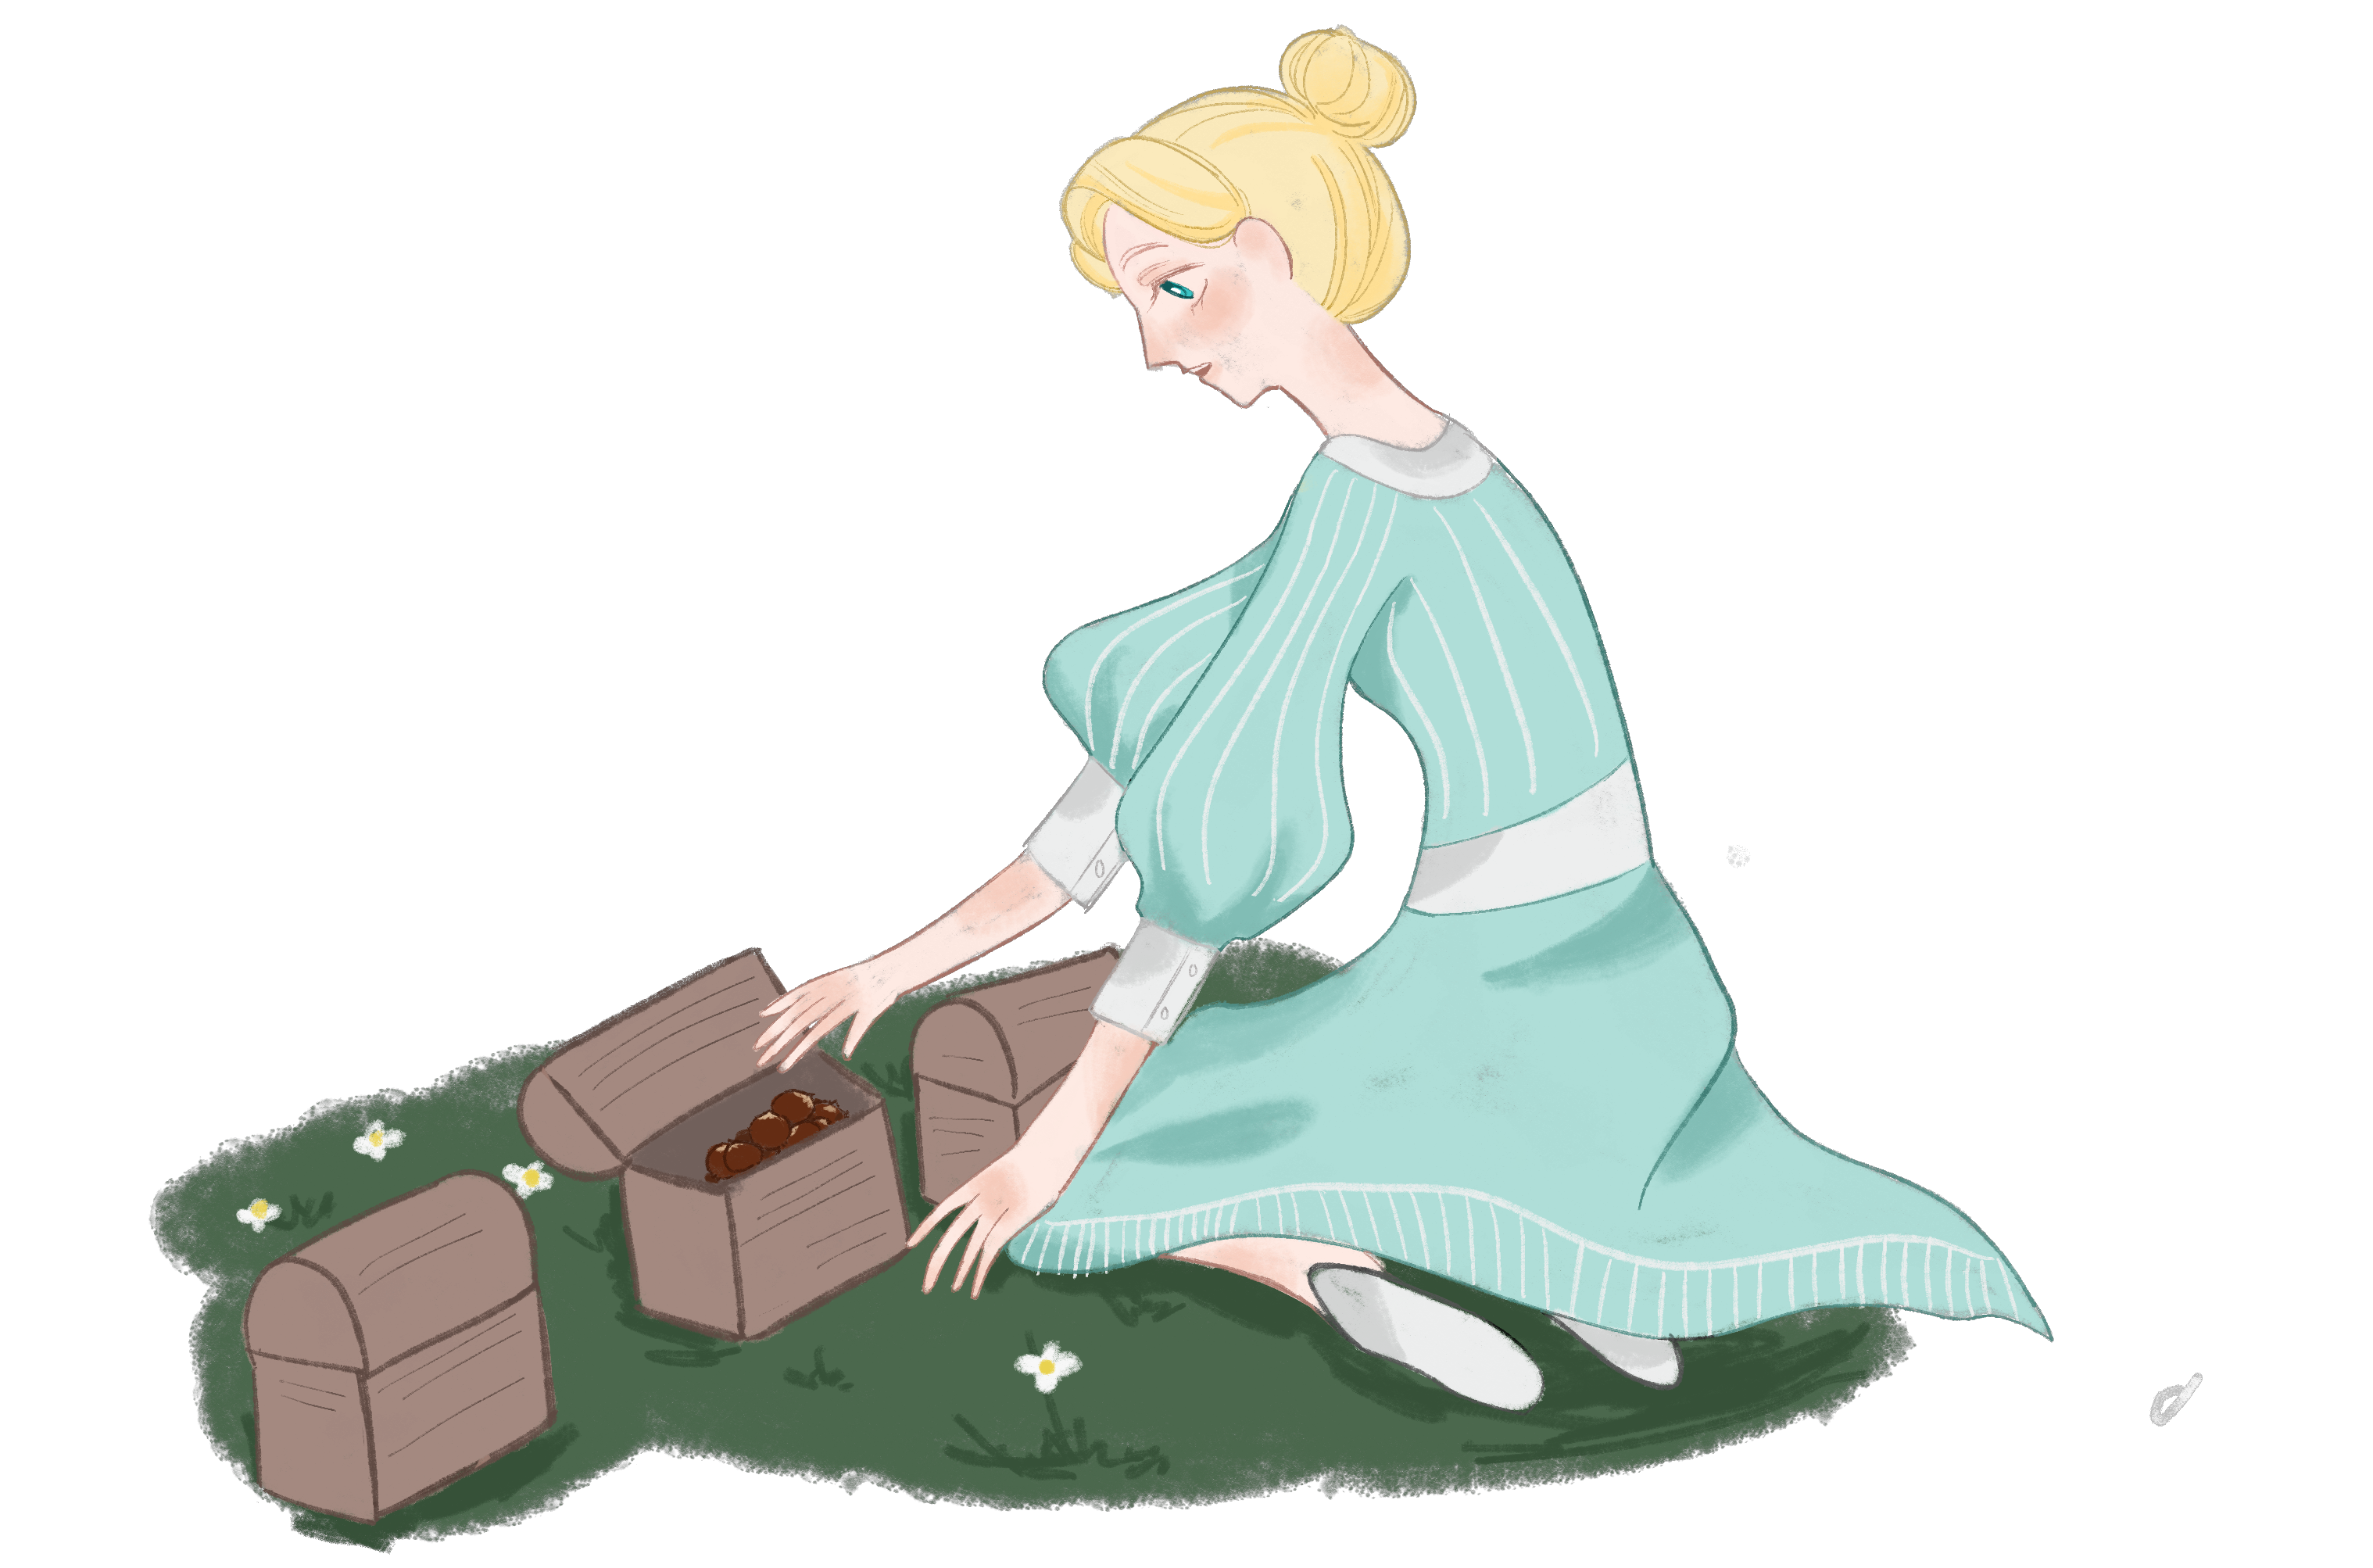
\includegraphics[width=1\linewidth]{Hinh1}
%		\vspace*{-20pt}
%	\end{figure}
%	$\pmb{2.}$ 	Lớp $6$A gồm $22$ bạn chia thành hai đội: Xanh gồm các bạn nam và Đỏ gồm các bạn nữ để tổ chức thi tài đối đáp, trả lời thông minh. Đầu tiên, bạn Hoa ở nhóm Đỏ đối đáp với $6$ bạn nam ở nhóm Xanh và giành chiến thắng. Tiếp theo, bạn Mai ở nhóm Đỏ đối đáp với $7$ bạn nam ở nhóm Xanh và cũng giành chiến thắng. Tiếp tục bạn Huệ ở nhóm Đỏ cũng chiến thắng $8$ bạn nam ở nhóm Xanh. Cứ tiếp tục như vậy, cuối cùng bạn Hà ở nhóm Đỏ đã đối đáp thông minh với toàn bộ các bạn nam ở nhóm Xanh và giành chiến thắng chung cuộc. Hỏi trong lớp có tất cả bao nhiêu bạn nam?
%	\begin{figure}[H]
%		\centering
%		\vspace*{-5pt}
%		\captionsetup{labelformat= empty, justification=centering}
%		
\includegraphics[width=1.01\linewidth]{Hinh2}
%		\vspace*{-5pt}
%	\end{figure}
%	$\pmb{3.}$ 	Có bốn chủ doanh nghiệp tới thăm trường học cũ của mình, mang theo một số món quà với dự định sẽ trao tặng cho các học sinh đang học ở đó. Khi tất cả $252$ em học sinh được mời xếp thành một hàng ngang, chủ doanh nghiệp thứ nhất tặng quà cho mỗi em đứng thứ tư trong hàng (các em ở số thứ tự $4,8,12,$ \ldots). Chủ doanh nghiệp thứ hai lại tặng quà cho mỗi em đứng thứ bảy (các em ở số thứ tự $7,14,21$, \ldots). Chủ doanh nghiệp thứ ba trao tặng quà cho mỗi em đứng thứ mười một (các em ở số thứ tự $11,22,33$, \ldots). Chủ doanh nghiệp thứ tư sẽ tặng quà cho các em còn lại. Hỏi có bao nhiêu em học sinh nhận được quà từ mỗi chủ doanh nghiệp?
%	\begin{figure}[H]
%		\centering
%		\vspace*{-5pt}
%		\captionsetup{labelformat= empty, justification=centering}
%		
\includegraphics[width=1\linewidth]{Hinh3}
%		\vspace*{-15pt}
%	\end{figure}
%	$\pmb{4.}$ 	Có ba nhà tài trợ quyết định giúp đỡ một tạp chí khoa học thường thức với tên gọi là Phi. Nhà tài trợ Quốc trao tặng một khoản tiền tính bằng dollar gồm có $4$ chữ số: $2$ chữ số đứng trước dấu phẩy, và hai chữ số sau dấu phẩy, trong đó số cent lẻ (tức là hai chữ số đứng sau dấu phẩy) bằng với đúng số dollar chẵn (tức là hai chữ số đứng trước dấu phẩy; ta nhớ lại $100$ cent $= 1$ dollar). Nhà tài trợ Minh tặng số tiền với số dollar chẵn lớn hơn $3$ dollar so với số dollar chẵn mà nhà tài trợ Quốc đã tặng nhưng số cent lẻ lại ít hơn $8$ lần số cent lẻ của nhà tài trợ Quốc. Nhà tài trợ Vũ hào phóng đem tặng số tiền bằng $1/7$ tổng số tiền của hai nhà tài trợ Quốc và Minh đã trao cộng lại. Hỏi số tiền ủng hộ của ba nhà tài trợ cho tạp chí Phi là bao nhiêu?
%	\begin{figure}[H]
%		\centering
%%		\vspace*{-5pt}
%		\captionsetup{labelformat= empty, justification=centering}
%		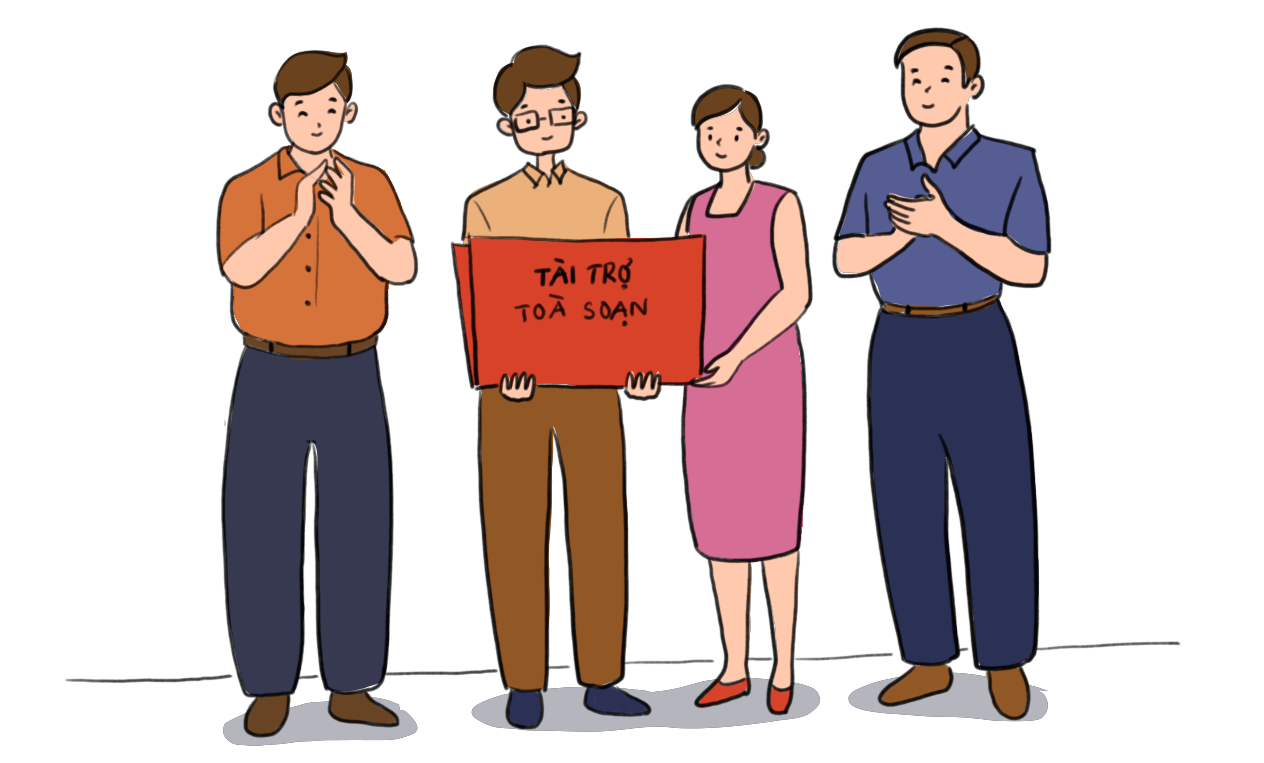
\includegraphics[width=0.8\linewidth]{Hinh4}
%		\vspace*{-10pt}
%	\end{figure}
%	\vskip 0.1cm
%	$\pmb{5.}$ 	Trên hòn đảo Ngọc ở giữa một đại dương xanh ngắt có $100$ thổ dân sinh sống, một số người trong họ luôn nói dối, còn những người còn lại luôn nói thật. Mỗi một thổ dân thờ phụng đúng một trong ba vị thần: thần Mặt trời, thần Mặt trăng hoặc thần Đất. Người ta hỏi mỗi thổ dân ba câu hỏi sau đây:
%	\begin{figure}[H]
%		\centering
%		\vspace*{-5pt}
%		\captionsetup{labelformat= empty, justification=centering}
%		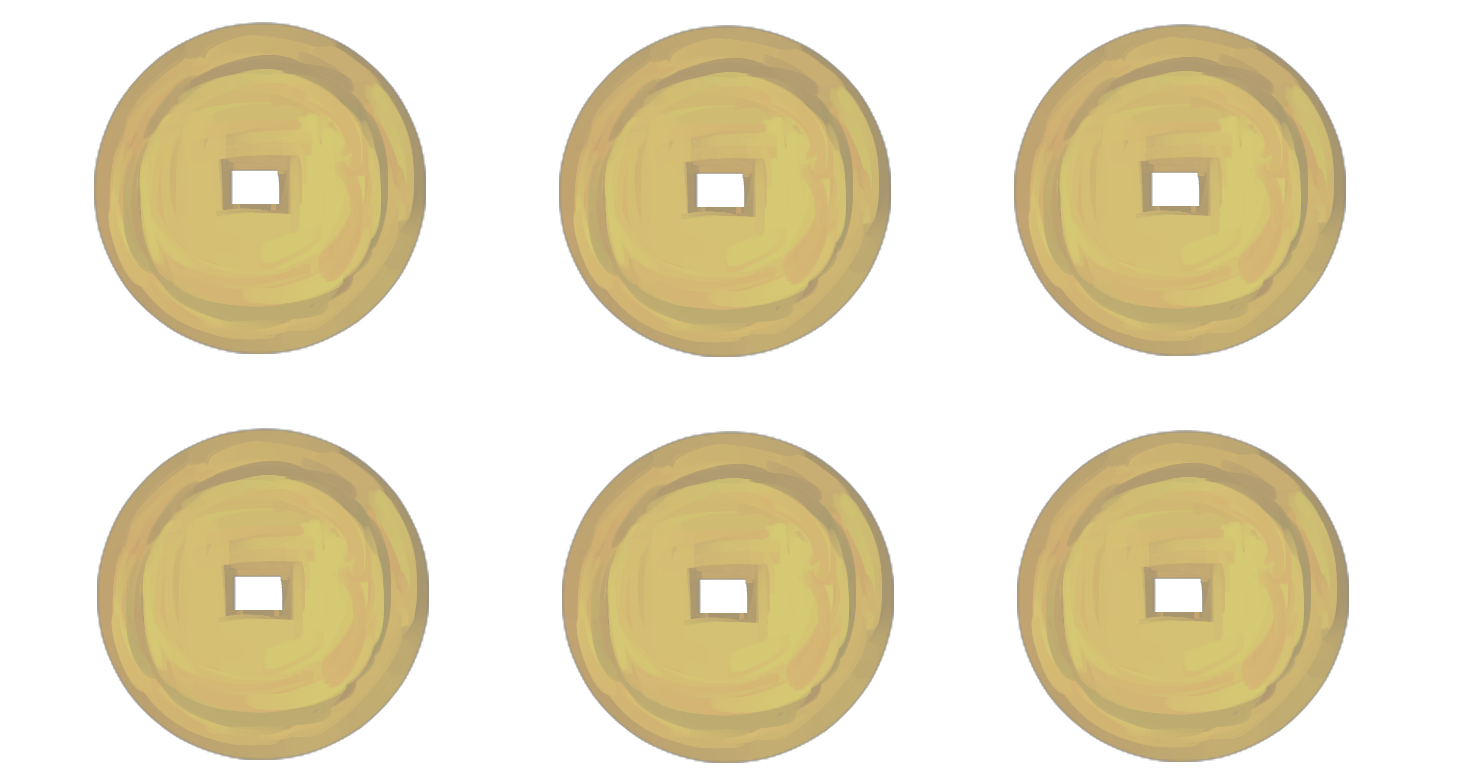
\includegraphics[width=1\linewidth]{Hinh5}
%		\vspace*{-20pt}
%	\end{figure}
%	$1.$ Ông (bà) có thờ phụng thần Mặt trời hay không?
%	\vskip 0.1cm
%	$2.$ Ông (bà) có thờ phụng thần Mặt trăng hay không?
%	\vskip 0.1cm
%	$3.$ Ông (bà) có thờ phụng thần Đất hay không?
%	\vskip 0.1cm
%	Có $60$ người trả lời khẳng định ``có" với câu hỏi thứ nhất, $40$ người trả lời khẳng định ``có" với câu hỏi thứ hai và $30$ người trả lời khẳng định ``có" với câu hỏi thứ ba. Hỏi trên đảo Ngọc có bao nhiêu thổ dân nói dối?
%	\vskip 0.1cm
%	$\pmb{6.}$ 	Có $100$ em học sinh được mời tới buổi tổng kết cuối năm học của nhà trường. Các ghế trong phòng họp được xếp ngay ngắn thẳng hàng theo dạng một hình vuông với $10$ dãy ghế, mỗi dãy có đúng $10$ chiếc ghế. Buổi họp phải diễn ra muộn hơn do bị cắt điện, vì thế các em học sinh bắt đầu bàn luận trao đổi với các bạn bên cạnh về kết quả điểm trung bình của mình. Em học sinh nào thấy trong tất cả những bạn ngồi kề sát mình: bên trái, bên phải, đằng sau, đằng trước và theo các đường chéo, chỉ có tối đa một bạn có điểm trung bình cao hơn hoặc bằng điểm trung bình của  mình, sẽ tự coi mình là ``có thành tích".
%	\begin{figure}[H]
%		\centering
%		\vspace*{-10pt}
%		\captionsetup{labelformat= empty, justification=centering}
%		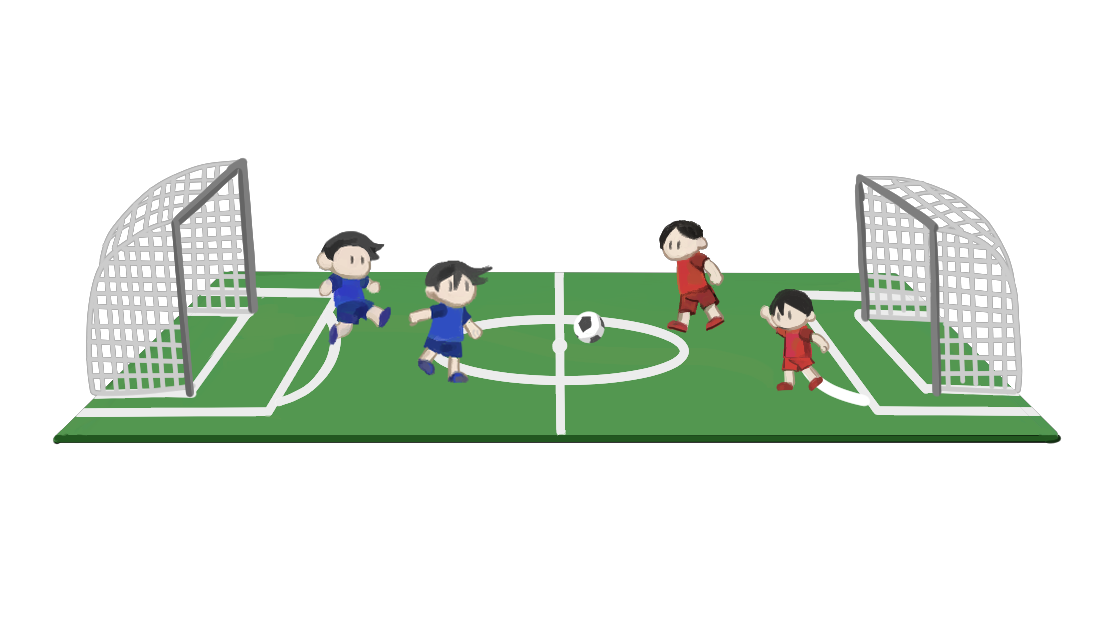
\includegraphics[width=0.85\linewidth]{Hinh6}
%		\vspace*{-10pt}
%	\end{figure}
%	Hỏi trong buổi họp đó có thể có tối đa bao nhiêu em học sinh đã tự coi mình là ``có thành tích" trong học tập?
%\end{multicols}
%\vspace*{-10pt}
%{\color{toancuabi}\rule{1\linewidth}{0.1pt}}
%\begingroup
%\AddToShipoutPicture*{\put(114,178){
\includegraphics[scale=1]{../tieude2.pdf}}} 
%\centering
%\endgroup
%\vspace*{75pt}
%
%\begin{multicols}{2}
%	$\pmb{1.}$ Các bạn nam mang kẹo tới lớp để tặng cho các bạn nữ. Bạn Phúc nói rằng mình đã mang tới đúng một nửa tổng số kẹo. Bạn Kiên nói rằng mình đã mang tới đúng một phần ba tổng số kẹo và chỉ chia kẹo của mình cho Mai và Tuyết, hơn nữa Mai được nhiều hơn so với Tuyết là $3$ chiếc kẹo. Em hãy chứng tỏ rằng có một bạn trong số Phúc và Kiên đã \linebreak nhầm lẫn.\\
%	\textit{Lời giải.} Giả sử cả hai bạn Phúc và Kiên đều không nhầm lẫn. Do Phúc không nhầm, nên tổng số kẹo được mang tới lớp phải là số chẵn (gấp $2$ lần số kẹo mà Phúc mang tới). Do Kiên cũng mang tới một số kẹo là số nguyên, bằng $1/3$ của một số chẵn, nên Kiên cũng mang tới một số kẹo là số chẵn. Theo lời của Kiên, số kẹo mà cậu đã tặng cho các bạn nữ là một số lẻ, do số kẹo mà Mai và Tuyết nhận được khác tính chẵn lẻ (hơn kém nhau là $3$ chiếc, mà $3$ là một số lẻ), mà tổng của hai số khác tính chẵn lẻ là một số lẻ. Ta nhận được mâu thuẫn. Suy ra có ít nhất một bạn nam trong số Phúc và Kiên đã nhầm lẫn.
%	\begin{figure}[H]
%			\centering
%		\vspace*{-5pt}
%		\captionsetup{labelformat= empty, justification=centering}
%		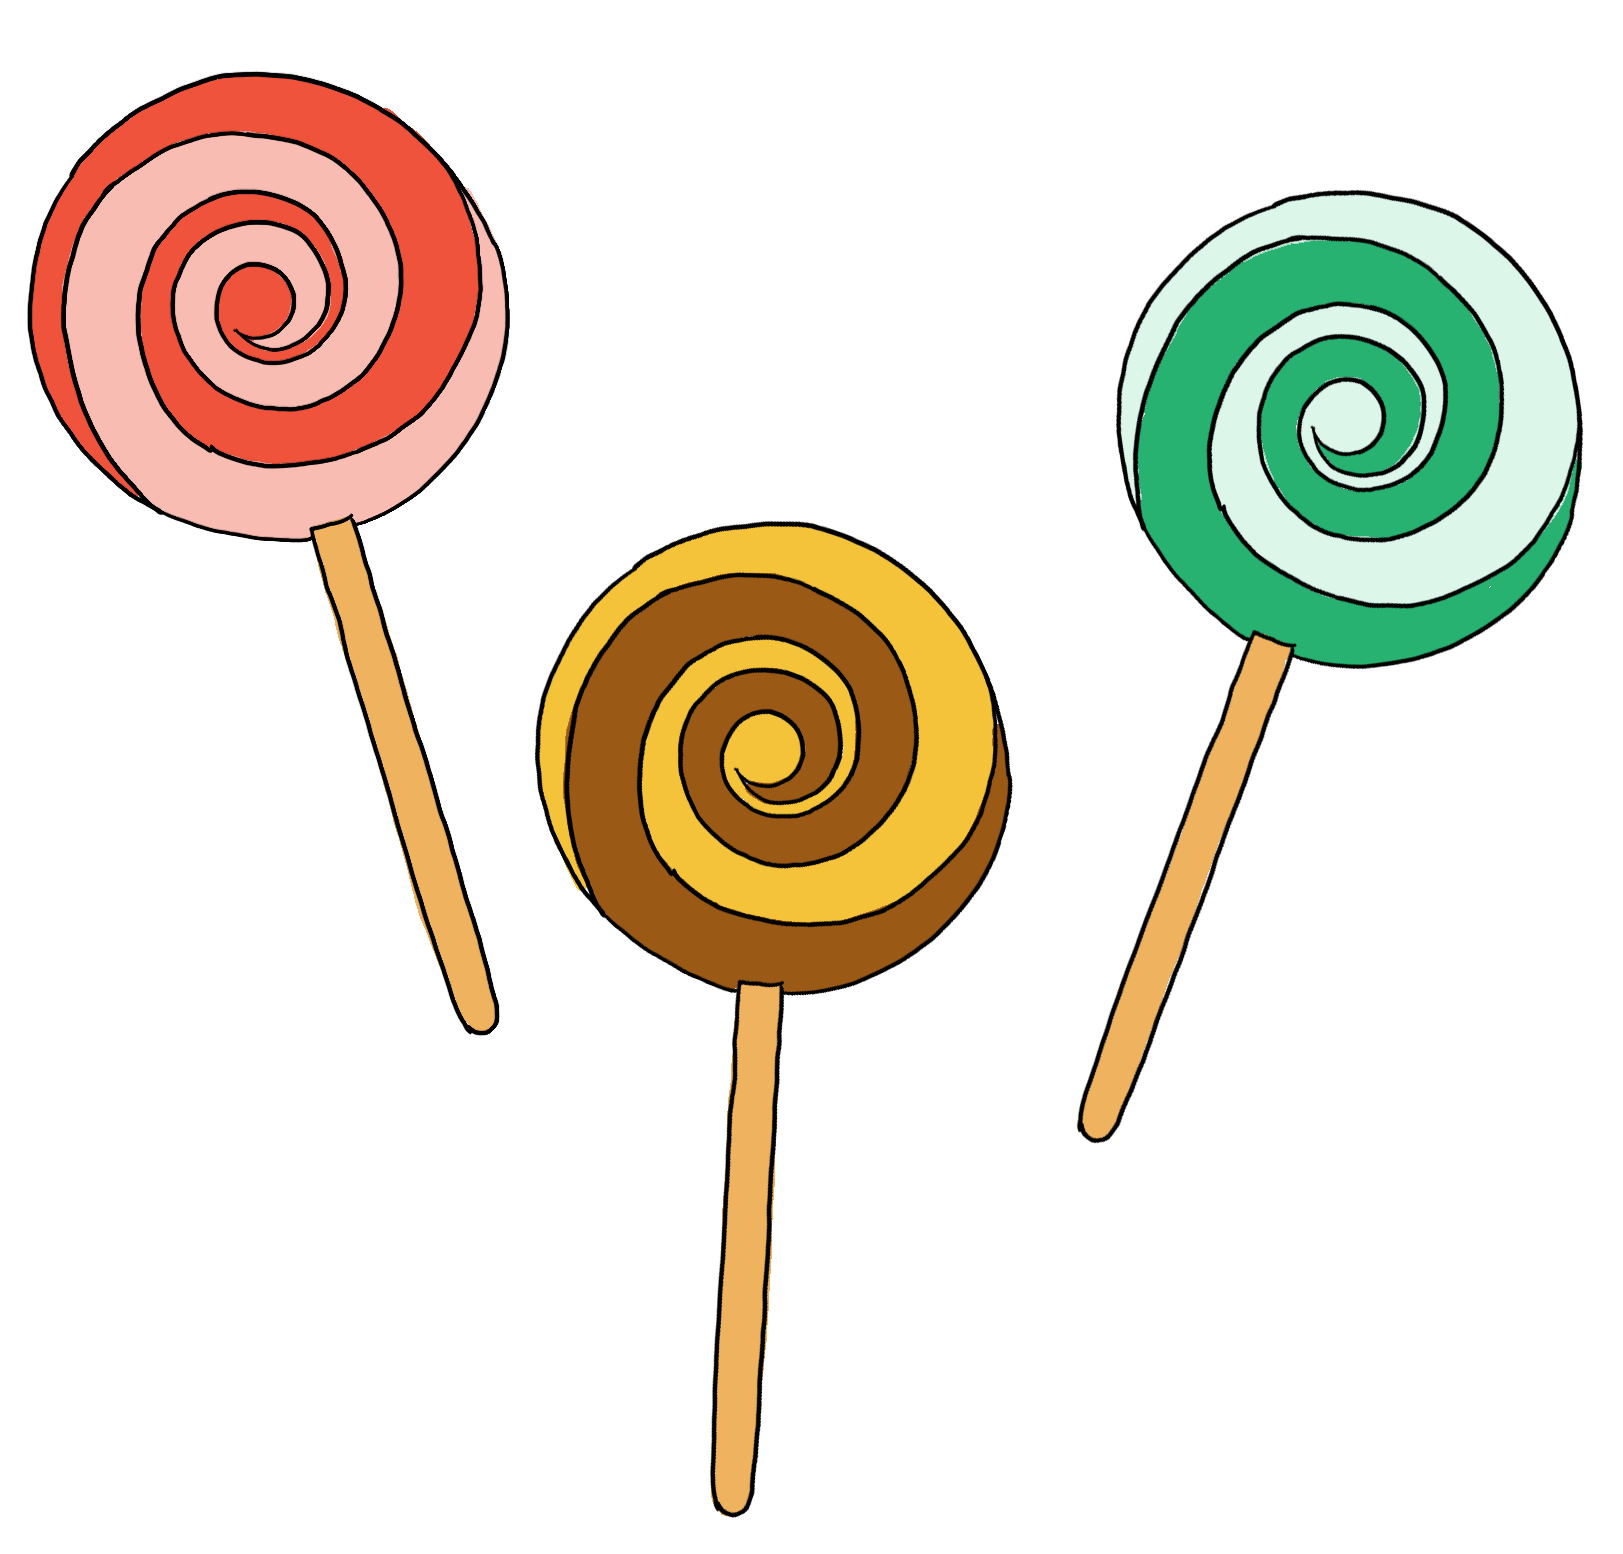
\includegraphics[width=0.6\linewidth]{Pi7_bai1}
%		\vspace*{-10pt}
%	\end{figure}
%	$\pmb{2.}$ Ba người thợ cùng đào một chiếc hố. Họ luân phiên lần lượt làm việc, mỗi người làm việc trong một thời gian nhất định. Nếu trong khi một người làm việc hai người còn lại cũng đồng thời đào hố thì hai người này sẽ đào được đúng một nửa hố. Hỏi nếu cả ba người cùng đồng thời đào thì họ sẽ làm nhanh hơn được bao nhiêu lần so với cách làm luân phiên ban đầu?
%	\begin{figure}[H]
%		\centering
%		\vspace*{-5pt}
%		\captionsetup{labelformat= empty, justification=centering}
%		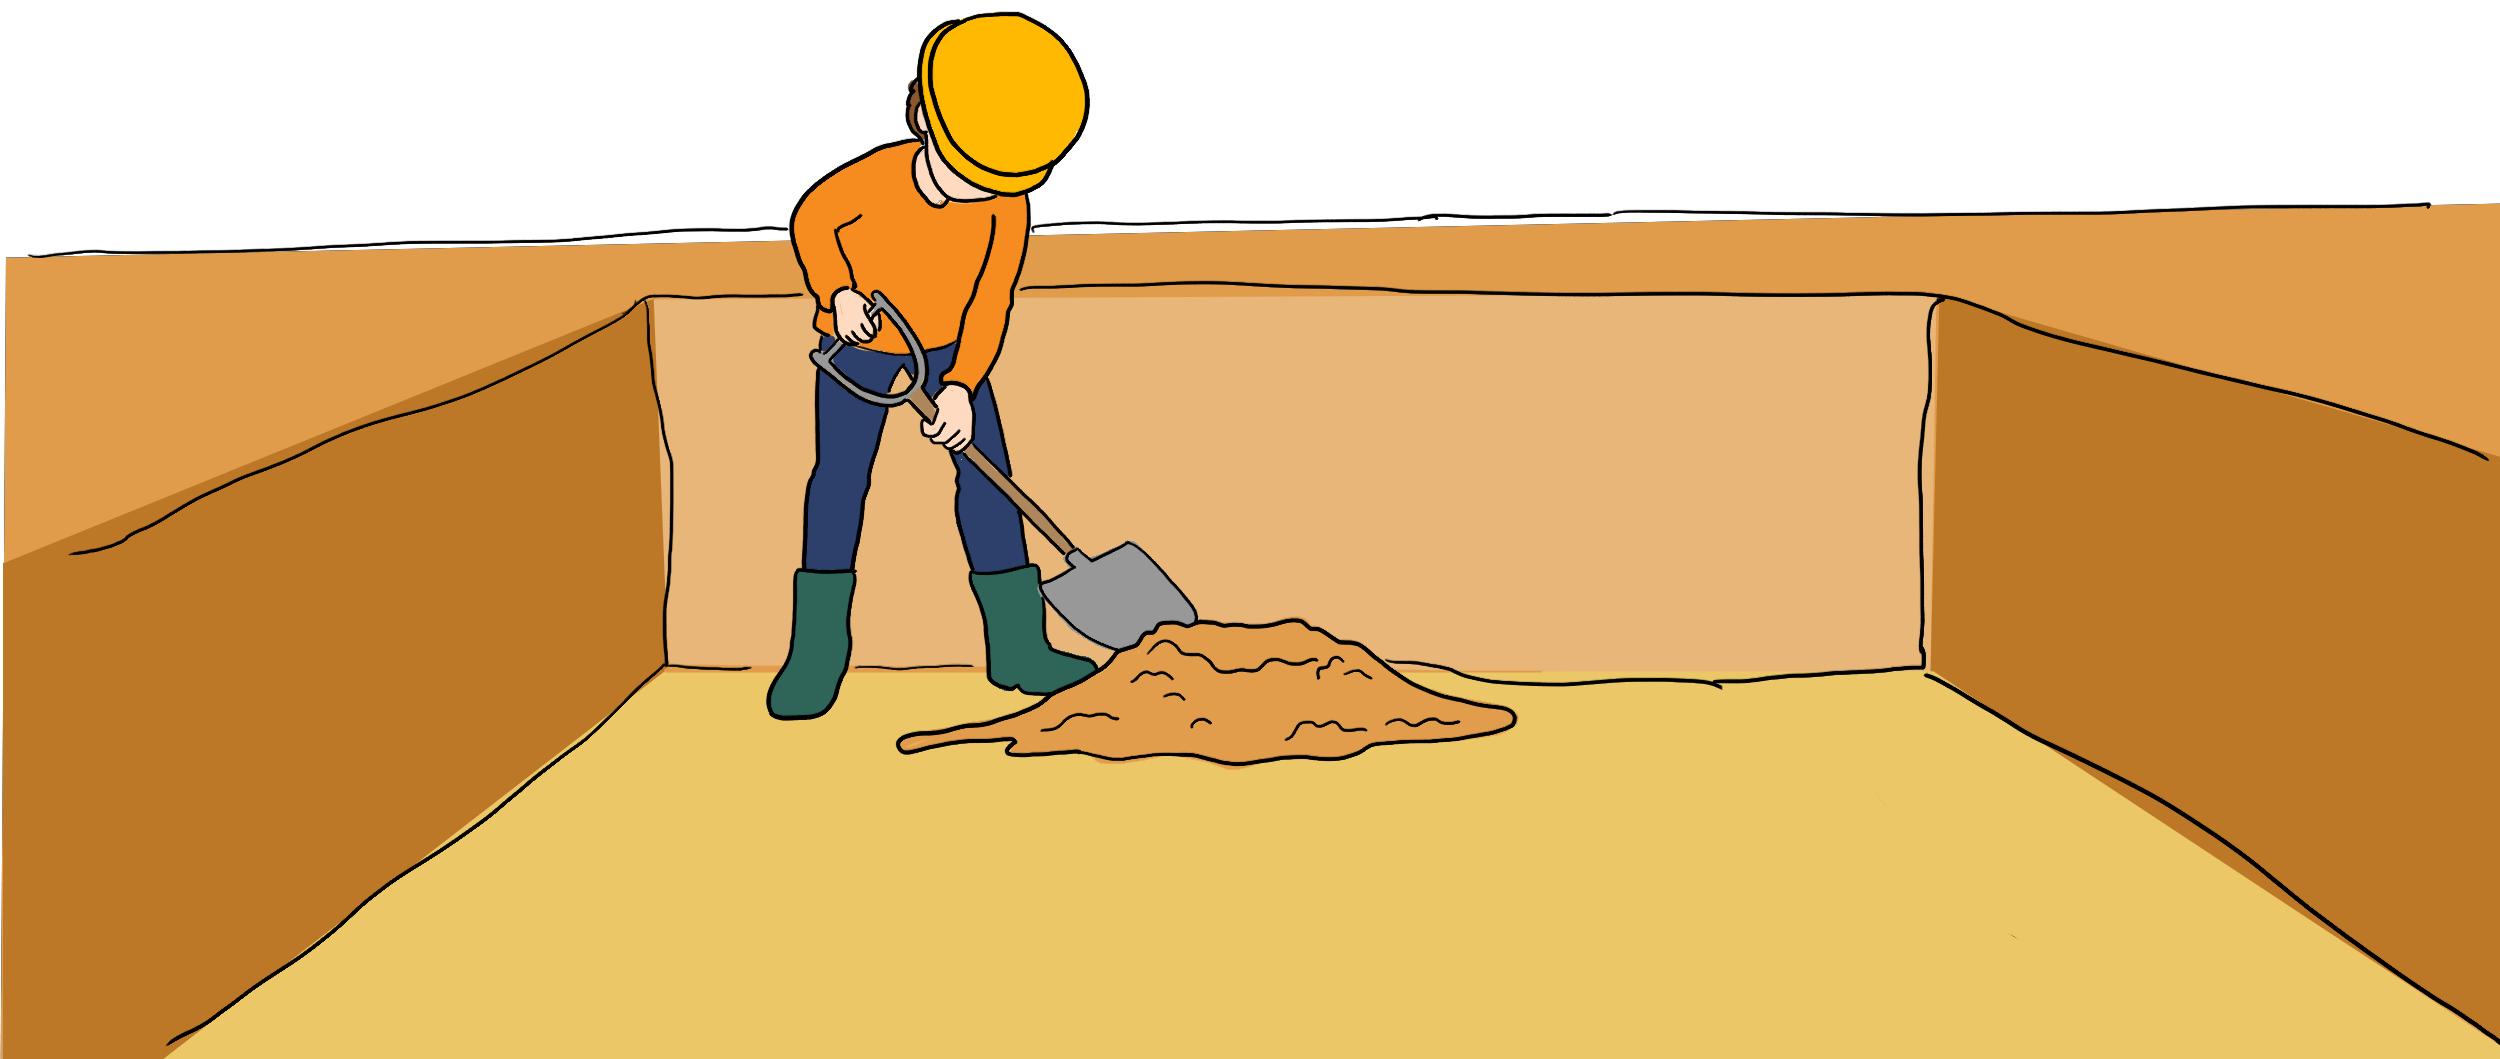
\includegraphics[width=1\linewidth]{Pi7_bai2}
%		\vspace*{-20pt}
%	\end{figure}
%	\textit{Lời giải.} 	Giả sử trong thời gian mỗi người đào ở chiếc hố ban đầu, hai người còn lại sẽ đi đào một chiếc hố bổ sung thêm khác. Như vậy khi kết thúc công việc, cùng với chiếc hố ban đầu, họ sẽ đào thêm được $3\cdot 0{.}5 = 1{.}5$ chiếc hố. Do đó, nếu cả ba người cùng làm công việc đào, thì trong cùng số thời gian như ban đầu, họ sẽ đào được $1+1{.}5=2{.}5$ (hố). Vậy, nếu cả ba người cùng đào thì họ sẽ làm nhanh hơn được $2{.}5$ lần so với cách đào luân phiên lần lượt như ban đầu.
%	\vskip 0.1cm
%	$\pmb{3.}$ Ba bạn Gấu, Thỏ và Mèo cùng quyết định xây một con đường từ nhà tới bờ suối với chiều dài $160m$. Các bạn thoả thuận sẽ đầu tư cho dự án mở đường quan trọng này với công sức đều như nhau. Cuối cùng khi dự án hoàn thành, hoá ra bạn Thỏ đã xây được $60$ mét đường, bạn Mèo xây được $100$ mét đường, còn bạn Gấu mải ngủ đông nên không xây được mét nào. Tuy nhiên, Gấu mang tới đóng góp bằng tiền cho dự án là $16$ triệu đồng từ số mật ong bán được của mình. Hỏi hai bạn Mèo và bạn Thỏ cần phải phân chia số tiền cho nhau như thế nào?
%	\begin{figure}[H]
%		\centering
%		\vspace*{-5pt}
%		\captionsetup{labelformat= empty, justification=centering}
%		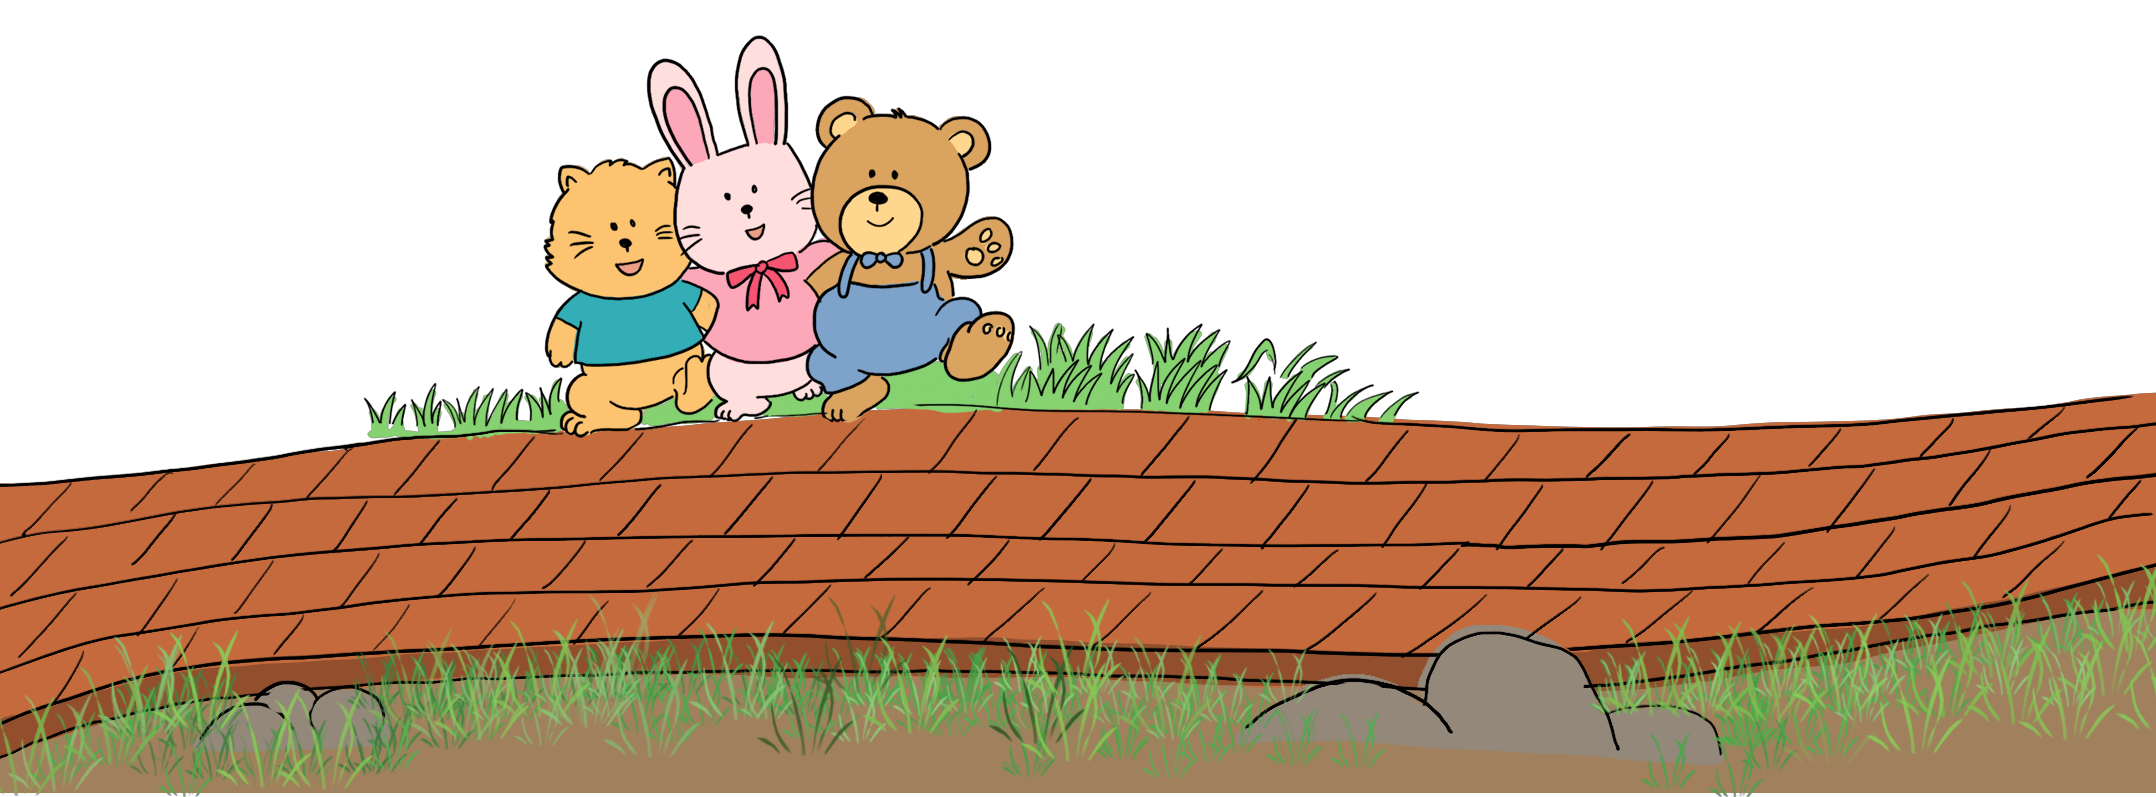
\includegraphics[width=1\linewidth]{Pi7_bai3}
%		\vspace*{-15pt}
%	\end{figure}
%	\textit{Lời giải.} 	Mỗi bạn theo kế hoạch phải xây đúng $\dfrac{160}{3} = 53\dfrac{1}{3}$  mét đường. Thỏ xây được $60$ (m) và Gấu xây được $100$ (m). Như vậy bạn Thỏ đã xây thay cho bạn Gấu số mét đường là
%	\begin{align*}
%		60 - 53 \frac{1}{3} = 6 \frac{2}{3}= \frac{20}{3} \text{ (m)},
%	\end{align*}
%	còn bạn Mèo đã xây thay cho bạn Gấu số mét đường
%	\begin{align*}
%		100- 53 \frac{1}{3} = 46 \frac{2}{3}=\frac{140}{3} \text{ (m).}
%	\end{align*}
%	Vì vậy số tiền mà bạn Gấu mang tới phải chia cho Thỏ và Mèo theo tỷ lệ $2: 14$, tức là Mèo được $14$ triệu đồng, còn Thỏ được $2$ triệu đồng từ số tiền đóng góp công sức của Gấu.
%	\vskip 0.1cm
%	$\pmb{4.}$ Bé Ly phải đi trồng hoa vào một hàng các chậu rất dài đặt thành hàng dọc ở công viên. Bé được giao nhiệm vụ là phải trồng hai loại hoa khác nhau vào hai chiếc chậu nếu giữa hai chậu này có đúng hai chiếc chậu, hoặc đúng ba chiếc chậu, hoặc đúng năm chiếc chậu khác. Hỏi bé Ly phải cần ít nhất bao nhiêu loại hoa để thực hiện được nhiệm vụ?
%	\begin{figure}[H]
%		\centering
%		\vspace*{-5pt}
%		\captionsetup{labelformat= empty, justification=centering}
%		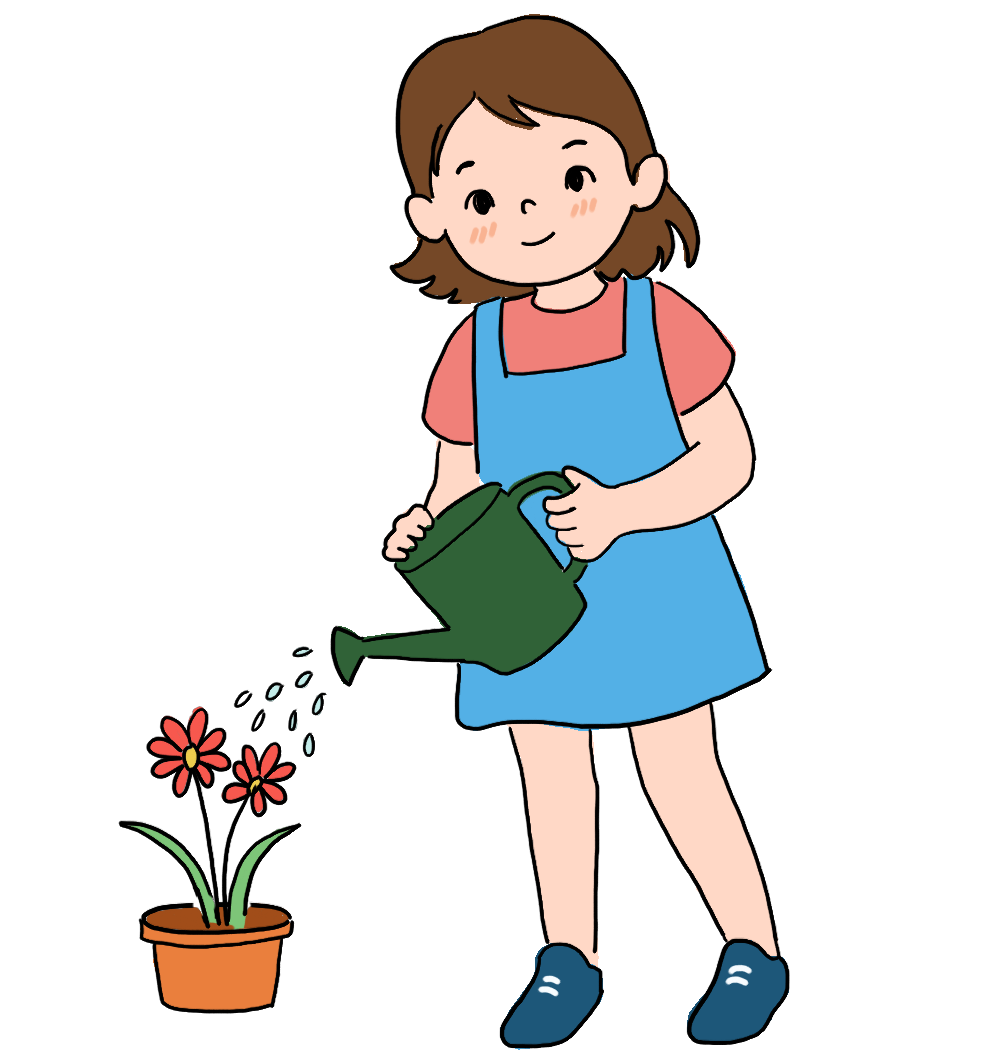
\includegraphics[width=0.45\linewidth]{Pi7_bai4}
%		\vspace*{-10pt}
%	\end{figure}
%	\textit{Lời giải.} Trước tiên ta thấy rằng bé Ly có thể chỉ cần $3$ loại hoa là thực hiện được nhiệm vụ. Thật vậy, giả sử Ly có $3$ loại là $A, B, C$. Khi đó nếu Ly trồng $3$ chậu đầu tiên trong hàng bằng loại $A$, $3$ chậu tiếp theo bằng loại $B$, $3$ chậu tiếp loại $C$ và lại $3$ chậu tiếp theo quay lại bằng loại $A$, vv \ldots thì rõ ràng yêu cầu đặt ra được thực hiện. 
%	\vskip 0.1cm
%	Bây giờ giả sử Ly chỉ có $2$ loại hoa là $A$ và $B$. Nếu Ly trồng ở chậu thứ nhất bằng hoa loại $A$ (không mất tính tổng quát), suy ra các chậu có số thứ tự tiếp theo là $4, 5, 7$ phải được trồng bằng hoa loại $B$. Nhưng khi đó giữa hai chậu số $4$ và số $7$ đều được trồng cùng loại hoa $B$ nhưng giữa chúng có đúng hai chậu khác là số $5$ và số $6$, suy ra mâu thuẫn với yêu cầu.
%	\vskip 0.1cm
%	Vậy Ly cần ít nhất $3$ loại hoa để trồng theo yêu cầu đặt ra.
%	 \vskip 0.1cm
%	$\pmb{5.}$ Trước một trận bóng đá giữa hai đội Xóm Đông và Xóm Bắc có $5$ dự đoán kết quả được đưa ra:
%	\vskip 0.1cm
%	$a)$	Sẽ không có tỷ số hoà;
%	\vskip 0.1cm
%	$b)$	Đội Xóm Đông sẽ bị thủng lưới;
%	\vskip 0.1cm
%	$c)$	Đội Xóm Bắc sẽ thắng;
%	\vskip 0.1cm
%	$d)$	Đội Xóm Bắc sẽ không thua;
%	\vskip 0.1cm
%	$e)$	Trong trận bóng sẽ có đúng $3$ bàn thắng được ghi.
%	\vskip 0.1cm
%	Sau khi trận bóng kết thúc, hoá ra chỉ có đúng $3$ dự đoán là chính xác. Vậy trận đấu đã kết thúc với tỷ số như thế nào?
%	\begin{figure}[H]
%		\centering
%%		\vspace*{-5pt}
%		\captionsetup{labelformat= empty, justification=centering}
%		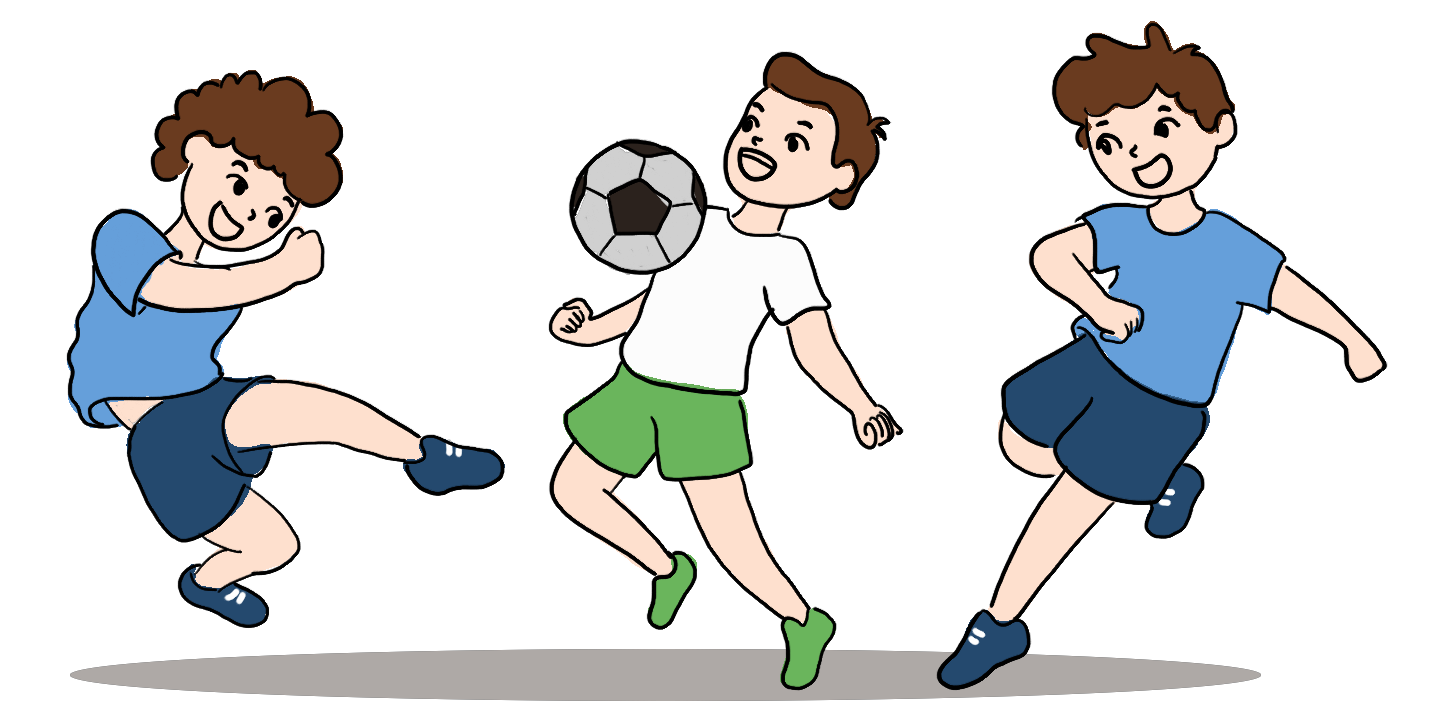
\includegraphics[width=0.85\linewidth]{Pi7_bai5}
%		\vspace*{-10pt}
%	\end{figure}
%	\textit{Lời giải.} Giả sử là đội Xóm Bắc thắng. Khi đó $4$ dự đoán $a)$, $b)$ $c)$ và $d)$ đều đúng, mâu thuẫn với điều kiện đặt ra.
%	\vskip 0.1cm
%	Tiếp theo, giả sử trận đấu kết thúc với tỷ số hoà. Khi đó ta lại có các dự đoán $a)$, $c)$ và $e)$ đều sai, điều này cũng mâu thuẫn với điều kiện đã cho.
%	\vskip 0.1cm
%	Vì vậy, trong trận bóng này đội Xóm Bắc đã thua. Khi đó các dự đoán $c)$ và $d)$ đều sai, và $3$ dự đoán còn lại là đúng. Có nghĩa là: trận đấu không có tỷ số hoà, có ít nhất một trái bóng được đưa vào lưới của đội Xóm Đông, và trong trận bóng có đúng $3$ bàn thắng được ghi. Điều đó có nghĩa là trận bóng kết thúc với tỷ số $1:2$ nghiêng về phía đội Xóm Đông.
%	\vskip 0.1cm
%	$\pmb{6.}$ 	Tại trại hè có $20$ em học sinh tham gia trò chơi Điệp viên tí hon diễn ra trong $2$ tuần. Mỗi Điệp viên tí hon sẽ theo dõi và viết báo cáo tỉ mỉ về sở thích cá nhân của $10$ em khác trong số $20$ em này để nộp cho Sở chỉ huy. Em hãy chứng tỏ rằng có ít nhất $10$ cặp Điệp viên tí hon đã theo dõi lẫn nhau và viết báo cáo về nhau.
%	\begin{figure}[H]
%		\centering
%		\vspace*{-5pt}
%		\captionsetup{labelformat= empty, justification=centering}
%		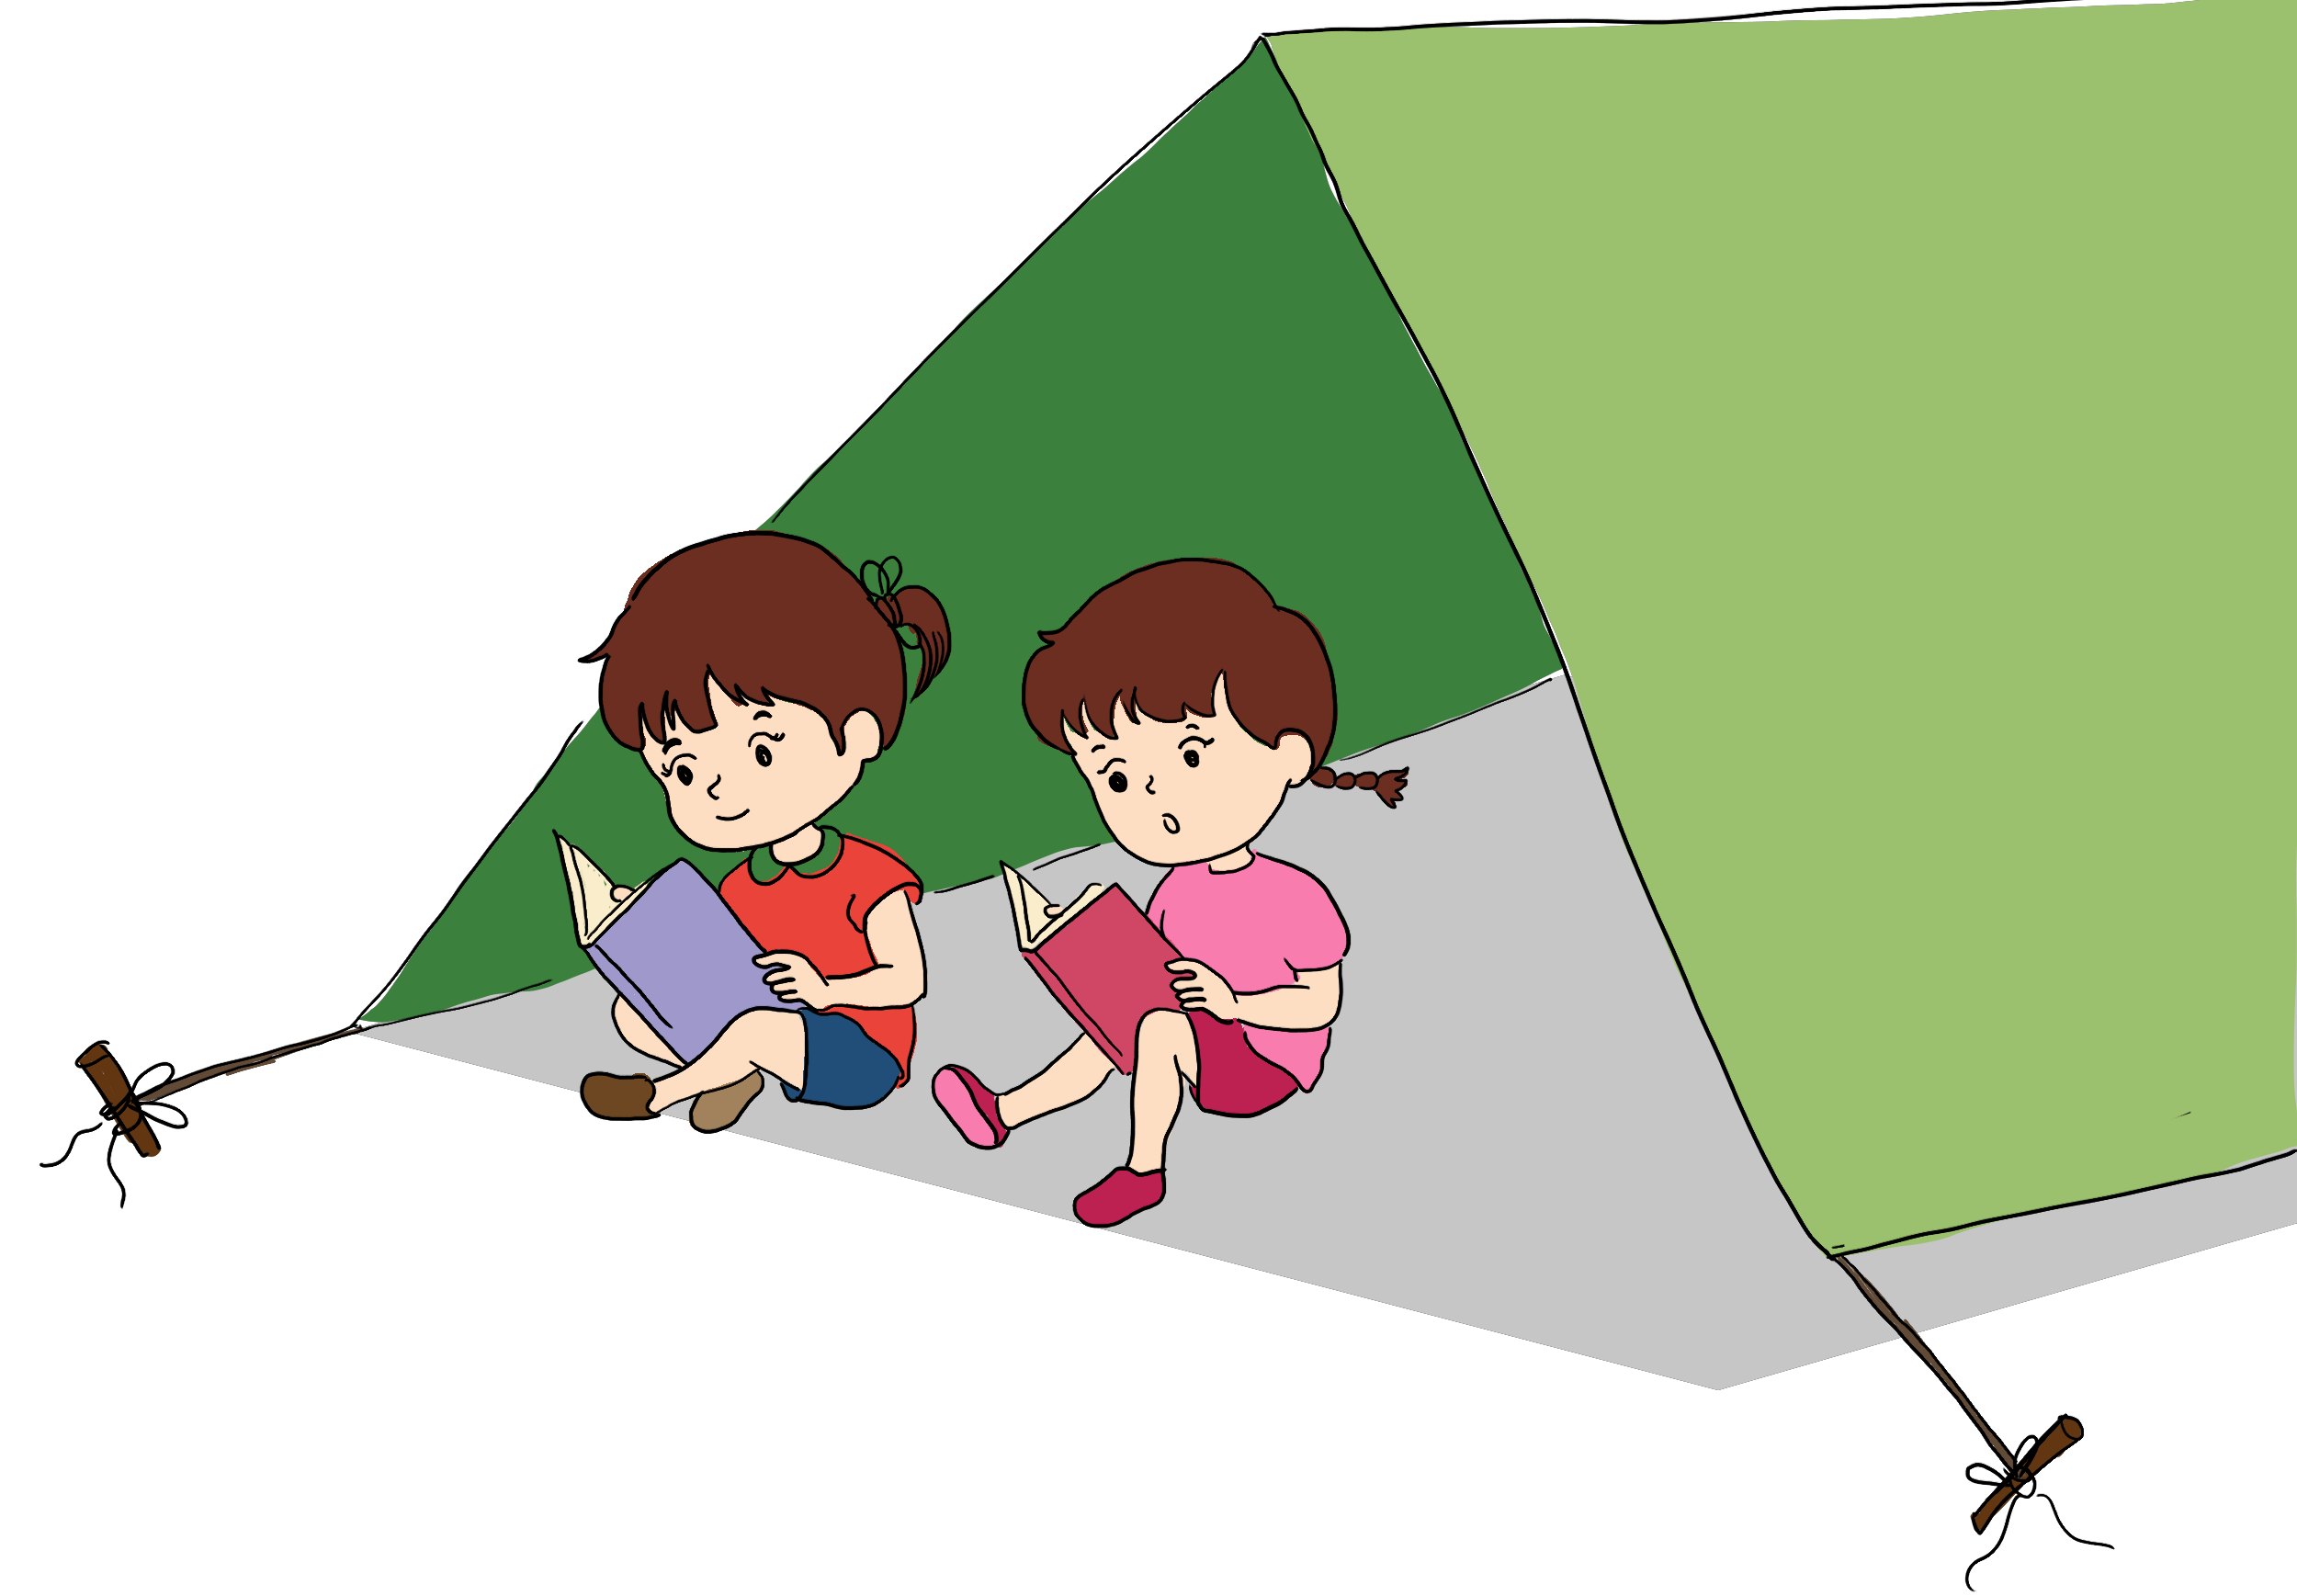
\includegraphics[width=0.75\linewidth]{Pi7_bai6}
%		\vspace*{-15pt}
%	\end{figure}
%	\textit{Lời giải.} Số các cặp Điệp viên tí hon là $\dfrac{20\times 19}{2} = 190$ (cặp). Có tất cả $10\times 20=200$ báo cáo được gửi về Sở chỉ huy vào cuối đợt chơi, suy ra phải có ít nhất $10$ cặp Điệp viên mà hai người trong mỗi cặp báo cáo lẫn nhau về Sở chỉ huy.
%\end{multicols}
%
%\newpage
%\begingroup
%\thispagestyle{toancuabinone}
%\blfootnote{$^1$\color{toancuabi}Ottawa, Canada.}
%\AddToShipoutPicture*{\put(60,733){
\includegraphics[width=17.2cm]{../mathc.pdf}}}
%%\AddToShipoutPicture*{\put(-2,733){
\includegraphics[width=17.2cm]{../mathl.pdf}}} 
%\AddToShipoutPicture*{\put(110,675){
\includegraphics[scale=1]{../tieudeb.pdf}}} 
%\centering
%\endgroup
%\vspace*{35pt}
%
%\begin{multicols}{2}
%	In this article, we discuss the Extremal Principle and its applications.
%	One of the simplest forms of the principle is as follow:
%	``in a finite set of numbers, there is a number with minimal value,
%	i.e. it is smaller than or equal to any other number in the set.
%	Similarly there is a number with maximal value,
%	i.e. it is larger than or equal to any other number in the set."
%	\vskip 0.1cm
%	\textit{Proof by contradiction} is an extremely useful tool when combining with the Extremal Principle,
%	as you will see in below examples.
%	\vskip 0.2cm
%	\PIbox{{\color{toancuabi}\textbf{\color{toancuabi}\color{toancuabi}Example} (Dancing at a party)}
%			At a party no boy danced with all the girls,
%			but each girl dances with at least one boy.
%			Prove that there are two pairs of girl--boy $(g_1, b_1)$ and $(g_2, b_2)$
%			who danced with each other but $g_1$ did not dance with $b_2$
%			and $g_2$ did not dance with $b_1.$}
%	\vskip 0.2cm
%	\textit{Solution.}
%		Let $b_1$ be \textit{the boy who danced with the maximum number of girls.}
%		Then there is a girl $g_2$ who he did not danced with.
%		For $g_2$ there is a boy $b_2$ that $(g_2,b_2)$ danced together.
%		Among the girls who danced with $b_1$ there is at least one $g_1$ who did not danced with $b_2,$
%		otherwise $b_2$ danced with $g_2$ and all the girls that $b_1$ danced with,
%		meaning $b_2$ danced with more girls than $b_1,$ contradicting with the choice of $b_1.$
%	\vskip 0.2cm
%	\PIbox{{\color{toancuabi}\textbf{\color{toancuabi}\color{toancuabi}Example} (Infinity by contradiction)}
%			$\Omega$ is a set of points on the plane.
%			Every point in $\Omega$ is a midpoint of two points in $\Omega$.
%			Show that $\Omega$ is infinite set.}
%	\vskip 0.2cm
%	\textit{Solution.}
%	Suppose that $\Omega$ is a finite set.
%	According to the Extremal Principle,
%	\textit{there exists two points $A, B \in \Omega,$ such that the distance $AB$ is maximal.}
%	\vskip 0.1cm
%	Now, since $B \in \Omega,$ there exist two points $C,D \in \Omega$ so that $B$ is the midpoint of $CD.$
%	\begin{figure}[H]
%			\vspace*{-5pt}
%			\centering
%			\captionsetup{labelformat= empty, justification=centering}
%			\begin{tikzpicture}[toancuabi,scale=0.75]
%					\draw  (0.,0.)-- (3.,3.);
%					\draw  (3.,3.)-- (5.,-3.);
%					\draw  (5.,-3.)-- (0.,0.);
%					\draw  (0.,0.)-- (4.,0.);
%						\draw [fill=white] (0.,0.) circle (1.5pt);
%						\draw (-0.32,0.11) node {$A$};
%						\draw [fill=white] (3.,3.) circle (1.5pt);
%						\draw (3.14,3.37) node {$C$};
%						\draw [fill=white] (5.,-3.) circle (1.5pt);
%						\draw (5.32,-3.01) node {$D$};
%						\draw [fill=white] (4.,0.) circle (1.5pt);
%						\draw (4.36,0.15) node {$B$};
%				\end{tikzpicture}
%			\vspace*{-10pt}
%		\end{figure}    
%	Since one of the angles $\angle ABC,$ $\angle ABD,$ says $\angle ABD$ is at least $90^{\circ},$
%	thus in $\triangle ABD,$ $AD > AB.$
%	This contradicts the assumption that $A, B$ are the two points in $\Omega,$ such that the distance $AB$ is maximal.
%	\vskip 0.1cm	
%	Thus, there are no such two points $A, B,$ so $\Omega$ is infinite set.
%	\vskip 0.2cm
%	\PIbox{{\color{toancuabi}\textbf{\color{toancuabi}\color{toancuabi}Example} (How many olives did the knights eat?)}
%		At the dinner of King Anthony, several knights sits around a round table eating green olives.
%		Minh, the Magician, made sure that each knight ate either twice as many olives
%		or $10$ olives less than his right neighbour. 
%		Is that possible that the knights could have eaten exactly $1001$ olives?}
%	\vskip 0.2cm
%	\textit{Solution.}
%	Let assume that the knights have eaten exactly $1001$ olives.
%	Let choose the knight who \textit{ate the smallest number of olives}.
%	(If there are some of them, choose one.)
%	His neighbour on the left, knight $k$, ate either $10$ less or twice more.
%	Since the knight we chose ate the smallest number of olives, then knight $k$ ate twice as many.
%	Therefore, knight $k$ ate an even number of olives. 
%	\vskip 0.1cm	
%	The neighbour on the left of knight $k$ ate either twice as many olives or $10$ olives less,
%	hence he ate an even number of olives as well. Making the full circle, we'll end us with the first knight,
%	who must have eaten an even number of olives as well.
%	\vskip 0.1cm	
%	Therefore, the total number of olives must be an even number.
%	The number of olives eaten cannot be $1001.$
%	\vskip 0.2cm
%	\PIbox{{\color{toancuabi}\textbf{\color{toancuabi}\color{toancuabi}Example} (Chop the flies)}
%		$25$ flies are resting on the outdoor table in the garden, waiting for lunch to be served.
%		It is known that for any three of them, two are at a distance less than $20$ cm;
%		and there are at least a pair of flies that are further than $20$ cm from each other.
%		\vskip 0.1cm
%		Minh's mother gave him a fly swatter, shown below, with a hoop of radius $20$ cm,
%		With a single strike he can swat the flies where the hoop landed.
%		In \textit{at least} how many strikes can he swat all of them?
%		\textit{Note that Minh is so fast that the flies do not have time for reaction during and between his lightning strikes.}}
%	\vskip 0.2cm
%	\begin{figure}[H]
%		\vspace*{-5pt}
%		\centering
%		\captionsetup{labelformat= empty, justification=centering}
%		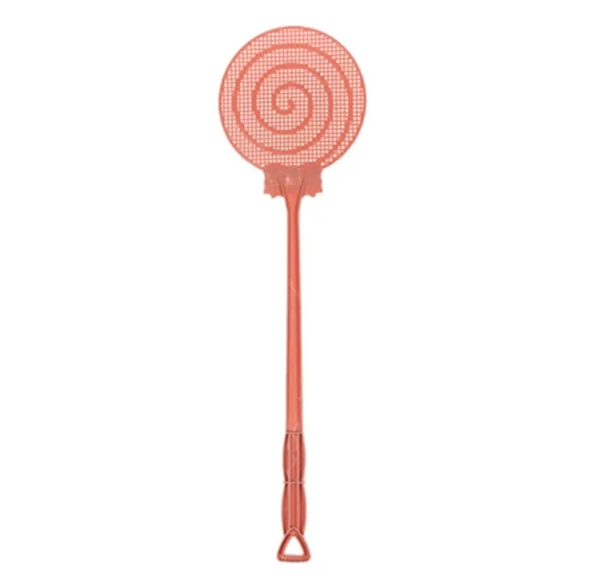
\includegraphics[width= 0.85\linewidth]{vr}
%		%		\caption{\small\textit{\color{}}}
%		\vspace*{-10pt}
%	\end{figure}
%	\textit{Solution.}
%	If no $2$ flies are further than $20$ cm from each other,
%	Minh can strike them all in $1$ strike by aiming the center of the swatter at any fly. 
%	But this is not the case, so let’s assume there are $2$ flies, $A$ and $B$, that are more than $20$ cm apart.
%	Then, every other fly is either in a $20$ cm radius of $A$ or in a $20$ cm radius of $B.$
%	Out of the $23$ remaining flies either at least $12$ will be in the $20$ cm radius of $A$
%	or $12$ will be in the $20$ cm radius of $B$.
%	Swatting that the $A$ or $B$ fly with the center of the swatter kills at least $13$.
%	\vskip 0.1cm
%	Thus, by $2$ strikes, he can swat them all.
%	\begin{center}
%		\textbf{\color{toancuabi}\color{toancuabi}Vocabulary}
%	\end{center}
%	{\color{toancuabi}Angle}: (dt) góc.
%	\vskip 0.1cm
%	{\color{toancuabi}Application}: (dt)  áp dụng, ứng dụng.
%	\vskip 0.1cm
%	{\color{toancuabi}Contradiction}: (dt) mâu thuẫn, {\color{toancuabi}proof by contradiction}: chứng minh bằng phản chứng.
%	\vskip 0.1cm
%	{\color{toancuabi}Even}: (tt) chẵn, {\color{toancuabi}even number}: số chẵn.
%	\vskip 0.1cm
%	{\color{toancuabi}Knight}: (dt) hiệp sỹ.
%	\vskip 0.1cm
%	{\color{toancuabi}Neighbour}: (dt) người bên cạnh. 
%	\vskip 0.1cm
%	{\color{toancuabi}Midpoint}: (dt) trung điểm.
%	\vskip 0.1cm
%	{\color{toancuabi}Discuss}: (đt) thảo luận, trao đổi.
%	\vskip 0.1cm
%	{\color{toancuabi}Distance}: (dt) khoảng cách.
%	\vskip 0.1cm
%	{\color{toancuabi}Fly}: (dt) côn trùng.
%	\vskip 0.1cm
%	{\color{toancuabi}Finite}: (tt) hữu hạn.
%	\vskip 0.1cm
%	{\color{toancuabi}Hoop}: (dt) vành, đầu vỉ ruồi.
%	\vskip 0.1cm
%	{\color{toancuabi}Infinite}: (tt) vô hạn, vô cùng, infinity (dt). 
%	\vskip 0.1cm
%	{\color{toancuabi}Maximal}: (tt) lớn nhất.
%	\vskip 0.1cm
%	{\color{toancuabi}Minimal}: (tt) nhỏ nhất.
%	\vskip 0.1cm
%	{\color{toancuabi}Olive}: (dt) quả ô-liu. 
%	\vskip 0.1cm
%	{\color{toancuabi}Plane}: (dt) mặt phẳng.
%	\vskip 0.1cm
%	{\color{toancuabi}Point}: (dt) điểm.
%	\vskip 0.1cm
%	{\color{toancuabi}Principle}: (dt) nguyên lý,  {\color{toancuabi}extremal principle}: nguyên lý cực hạn.
%	\vskip 0.1cm
%	{\color{toancuabi}Swatter}: vỉ, {\color{toancuabi}fly swatter}: vỉ ruồi.
%	\vskip 0.1cm
%	{\color{toancuabi}Set}: (dt) tập hợp.
%	\vskip 0.1cm
%	{\color{toancuabi}Strike}: (đt) đập, đánh.
%	\vskip 0.1cm
%	{\color{toancuabi}Table}: (dt) cái bàn, {\color{toancuabi}round table}: bàn tròn, {\color{toancuabi}outdoor table}: bàn ngoài trời.
%	\vskip 0.1cm
%	{\color{toancuabi}Value}: (dt) giá trị.
%	
%\end{multicols}
